\documentclass{article}
\usepackage{../AMadhava}
\rhead{MAT 533: Analysis II Notes}
\setcounter{secnumdepth}{0}
\usepackage{pgfplots,mathtools}
\pgfplotsset{compat=newest}
\def\xmax{1}\def\ymax{1.2}
\usepackage{scalerel,stackengine}
\stackMath
\renewcommand\wh[1]{%
	\savestack{\tmpbox}{\stretchto{%
			\scaleto{%
				\scalerel*[\widthof{\ensuremath{#1}}]{\kern-.6pt\bigwedge\kern-.6pt}%
				{\rule[-\textheight/2]{1ex}{\textheight}}%WIDTH-LIMITED BIG WEDGE
			}{\textheight}% 
		}{0.5ex}}%
	\stackon[1pt]{#1}{\tmpbox}%
}
%\usepackage{amsfonts}
\fontsize{11.9pt}{2cm}\selectfont


\title{Lecture Notes in Analysis II}
\author{\me}
\date{Spring 2026}
\begin{document}
	\maketitle
	\fullline 
	\tableofcontents
	\halfline 
	\newpage 
	
	
\section{Lecture 1: Normed Linear Spaces and Completeness}
\subsubsection{Key Topics:}
(1) Linear Spaces, (2) Norms, (3) Normed Linear Spaces, (4) Banach Spaces
\subsubsection{Summary:}
In this lecture, we will define the notion of a \textit{norm} on a linear space $X$, investigate the convergence of sequences in normed linear spaces, and define what it means for a normed linear space to be complete (or \textit{Banach}). We will also look at a few examples. 
\subsubsection{Lecture:}
\begin{itemize}
	\item \textbf{Def. (Normed Linear Space)} Let $X$ be a linear space over some field $K$. A \textit{norm} on $X$ is a map $\norm{\empspace}: X \to [0,\infty)$ with the following properties: 
	\begin{enumerate}[itemsep =-2pt,label = (\arabic{*})]
		\item $\norm{x} \geq 0$ for all $x \in X$, with equality iff $x = 0$ (positivity)
		\item $\norm{x + y} \leq \norm{x} + \norm{y}$ for all $x, y \in X$ (triangle inequality)
		\item $\norm{cx} = \abs{c}\norm{x}$ for all $c \in K$, $x \in X$ (homogeneity).
	\end{enumerate}
	\item \textbf{Ex. 0. (Norms on Euclidean Space)} Let $X = \mathbb{R}^{n}$. There exist various different norms on $X$: 
	\begin{enumerate}[itemsep =-2pt, label = (\arabic{*})]
		\item (Euclidean Norm): Let $x \in X$, and define the map $\norm{\empspace}: X \to [0, \infty)$ as follows: 
		\begin{equation}
			\norm{x} = \left(\sum_{1}^{n}\abs{x_{i}}^{2}\right)^{1/2}. 
		\end{equation}
		(Note that this is the $\ell^{2}$-norm). 
		\item ($\ell^{p}$-Norms): Let $1 \leq p < \infty$. Then the map $\norm{\empspace}_{p}: X \to [0,\infty)$ defined by 
		\begin{equation}
			\norm{x}_{p} = \left(\sum_{1}^{n}\abs{x_{i}}^{p}\right)^{1/p}
		\end{equation}
		is a norm on $X$; note that the same map for $p < 1$ is \textit{not} a norm since the triangle inequality is not satisfied. Indeed, for $p < 1$, $\norm{x + y}_{p} \geq \norm{f}_{p} + \norm{g}_{p}$. 
		\item ($\ell^{\infty}$-Norm): For $p = \infty$, let $\norm{\empspace}_{\infty}: X \to [0,\infty)$ be the map defined by 
		\begin{equation}
			\norm{x}_{\infty} = \max_{1 \leq i \leq n}\abs{x_{i}}. 
		\end{equation}
	\end{enumerate}
	The shape of the unit ball in $\mathbb{R}^{n}$ depends on the norm we consider. For instance, when $n = 2$, Figure \ref{fig:lect1_norms} shows the possible shapes. 
	\begin{figure}[h!]
		\centering
		\begin{tikzpicture}
			\draw[Stealth-Stealth] (-6,-2) -- (-6,2); \draw[Stealth-Stealth] (-8,0) -- (-4,0); \draw[fill=none] (-6,0) circle (1);
			\draw[Stealth-Stealth] (0,-2) -- (0,2); \draw[Stealth-Stealth] (-2,0) -- (2,0); \draw[-] (1,0) -- (0,1) -- (-1,0) -- (0,-1) -- cycle;
			\draw[Stealth-Stealth] (6,-2) -- (6,2); \draw[Stealth-Stealth] (4,0) -- (8,0); 
			\draw[-] (7,1) -- (5,1) -- (5,-1) -- (7,-1) -- cycle;
		\end{tikzpicture}
		\caption{Unit ball in $\mathbb{R}^{2}$ in different norms: from left to right, (a) Euclidean norm, (b) $\ell^{1}$-norm, (c) $\ell_{\infty}$-norm.}
		\label{fig:lect1_norms}
	\end{figure}
	\item \textbf{Ex. 1. ($L^{1}$-Norms)} Let $X = C^{\infty}([0,1])$. For $f \in X$, define $\norm{f} = \int_{0}^{1}\abs{f}\;dx$. Then this is the $L^{1}$-norm on $X$. 
	\item \textbf{Ex. 2. (Polynomial Norms)} Let $X$ be the set of all finite-degree polynomials in one variable. Then define a norm on $X$ as follows: for each $P = \sum_{0}^{n}a_{i}x^{i} \in X$, let 
	\begin{equation}
		\norm{P} = \sum_{0}^{n}\abs{a_{i}}. 
	\end{equation}
	\item \textbf{Def. (Cauchy Sequences)} Let $(X, \norm{\empspace})$ be a normed linear space. A sequence is a function $\mathbb{N} \to X$, and is denoted by $\{x_{n}\}_{1}^{\infty} = (x_{1}, x_{2}, \ldots)$. A sequence is said to be \textit{Cauchy} iff $\norm{x_{n} - x_{m}} \to 0$ as $n,m \to \infty$. 
	\item \textbf{Def. (Complete Space)} Let $X$ be a normed linear space. $X$ is said to be complete if every Cauchy sequence in $X$ converges in $X$. 
	\item \textbf{Ex. 0. (Finite-Dimensional Normed Spaces)} Every finite-dimensional normed linear space is complete. 
	\item \textbf{Ex. 1. ($C^{\infty}([0,1])$ is Incomplete)} Let $X = C^{\infty}([0,1])$, and let $X$ have the $L^{1}$-norm. Then $(X, \norm{\empspace}_{1})$ is incomplete. Intuitively, this is because non-smooth functions can be uniformly approximated by smooth functions: 
	\begin{figure}[h!]
		\centering
		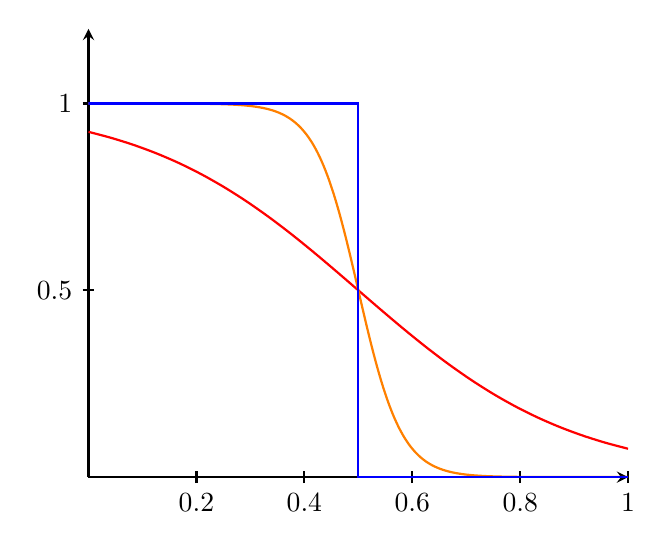
\begin{tikzpicture}
			\begin{axis}[
				domain=0:\xmax,ymax=\ymax,
				ytick={0.5,1},
				smooth,thick,
				axis lines=center,
				every tick/.style={thick},
				legend cell align=left]
				
				% Graphs
				\def\chempot{1}
				\def\n#1{1/(e^(#1*(x - \chempot+0.5)) + 1)}
				\addplot[color=red]{\n{5}};
				\addplot[color=orange,samples=100]{\n{25}};
				\addplot[const plot,color=blue] coordinates {(0,1) (\chempot-0.5,0) (\xmax,0)};
			\end{axis}
		\end{tikzpicture}
		\caption{Approximation of a non-smooth function by smooth functions. Note that the red function should be supported in $[0,1]$.}
		\label{fig:cinfty_not_complete}
	\end{figure}
	\item \textbf{Ex. 2. (Discrete Space is Incomplete)} Let $X$ be the space of real-valued sequences that only have finitely many nonzero terms. Define the norm $\norm{\{a_{n}\}} \coloneqq \sum \abs{a_{n}}$. Then $(X, \norm{\empspace})$ is incomplete. 
\end{itemize}

\section{Lecture 4: Weak and Strong Convergence}
\subsubsection{Key Topics:}
(1) Weak and Strong Convergence, (2) Compactness of the Unit Ball, (3) Riesz's Theorem, (4) Kakutani's Theorem 
\subsubsection{Summary:}
In this lecture, we will see a couple of different compactness results. In particular, we will study strong and weak compactness, and show that strong compactness is, in general, impossible to attain. We will see applications of these convergence types to the unit ball and reflexive spaces. 
\subsubsection{Lecture:}
\begin{itemize}
	\item \textbf{Thm. (Riesz's Theorem)} Let $X$ be a normed linear space. Then the unit ball $\{x \in X: \norm{x} \leq 1\}$ is compact if and only if $\dim(X) < \infty$.
	
	\begin{solutions}
		($\Leftarrow$) Suppose $X$ is a finite-dimensional space. In HW 2, we showed that every norm on $X$ is equivalent, and so is equivalent to the Euclidean norm. This means that the induced topology is the same as the Euclidean topology on $X$. Then since the unit sphere is closed and bounded in the Euclidean norm, by the Heine-Borel Theorem\footnote{\href{http://math.stackexchange.com/questions/4959961/heine-borel-for-finite-dimensional-normed-vector-spaces}{http://math.stackexchange.com/questions/4959961/heine-borel-for-finite-dimensional-normed-vector-spaces}}, we conclude that the unit sphere is compact. 
		
		($\Rightarrow$) Suppose that $\dim(X) = \infty$. We wish to show that the unit sphere is not compact; since $X$ is a normed (hence, metric) space, equivalence of sequential compactness and compactness implies it is sufficient to find a sequence with no convergent subsequence. In particular, we will construct a sequence $\{x_{j}\} \subseteq \{\norm{x} \leq 1\}$ so that $\norm{x_{j} - x_{k}}\geq \frac{1}{2}$ for all $j\neq k$. We proceed by induction. Choose $x_{1} \in X$ with $\norm{x_{1}} = 1$. Suppose that we have chosen $x_{1}, \ldots, x_{n}$ with $\norm{x_{j}}\leq 1$ for all $j = 1, 2,\ldots, n$, and $\norm{x_{j} - x_{k}}\geq \frac{1}{2}$ for $j \neq k$. Let $P = \operatorname{span}\{x_{1}, \ldots, x_{n}\}$. Since $P \subsetneq X$, there exists some $y_{n + 1} \in X\setminus P$ so that $\norm{y_{n + 1}}\leq \frac{1}{4}$. Let $\delta$ be the distance between $y_{n + 1}$ and $P$: 
		\begin{equation}
			\delta = \inf_{x \in P}\norm{y_{n + 1} - x} > 0. 
		\end{equation}
		In particular, there exists some $x_{\ast} \in P$ so that $\norm{y_{n + 1} - x_{\ast}} \leq (11/10)\delta$. Define the element 
		\begin{equation}
			x_{n + 1} = \frac{1}{2}\cdot \frac{y_{n + 1} - x_{\ast}}{\delta}. 
		\end{equation}
		We observe the following: 
		\begin{enumerate}[itemsep =-2pt,label = (\roman{*})]
			\item $\displaystyle \norm{x_{n + 1}} = \frac{1}{2\delta}\norm{y_{n + 1} - x_{\ast}} \leq \frac{1}{2\delta} \cdot \frac{11\delta}{10} = \frac{11}{20} < 1$. Hence, $x_{n + 1} \in \{\norm{x} \leq 1\}$. 
			\item For any $j \leq n$, 
			\begin{align}
				\begin{split}
					\norm{x_{n + 1} - x_{j}} &= \norm{\frac{y_{n + 1} - (x_{\ast} + 2\delta x_{j})}{2\delta}} \geq \frac{\delta}{2\delta} = \frac{1}{2}, 
				\end{split}
			\end{align}
			where the inequality follows from the fact that $x_{\ast} + 2\delta x_{j} \in P$. 
		\end{enumerate}
		Hence, we continue building $\{x_{j}\}$ in this way; by construction, this sequence has no convergent subsequence, which proves that the unit ball cannot be compact. 
	\end{solutions}
	\item \textbf{Rmk.} Riesz's theorem shows the problem with \textit{strong} convergence. Over the following results, we will demonstrate that \textit{weak} convergence is better for compactness. Our goal is to show that the unit ball is weakly compact in an arbitrary reflexive space. 
	\item \textbf{Def. (Weak Convergence)} Let $X$ be a normed linear space, and $X^{\ast}$ its dual space. $\{x_{n}\}_{n = 1}^{\infty} \subseteq X$ converges \textit{weakly} to $x \in X$ if for all $\ell \in X^{\ast}$, $\ell(x_{n})$ converges to $\ell(x)$. Let's recall a few results we had from last time $\ldots$
	\item \textbf{Prop. (Norm for Weak Convergence)} Let $X$ be a normed linear space, and assume $x_{n}$ converges to $x$ weakly. Then the following are true: 
	\begin{enumerate}[itemsep =-2pt,label = (\roman{*})]
		\item $\sup\limits_{n}\norm{x_{n}} < \infty$, 
		\item $\norm{x} \leq \liminf\limits_{n}\norm{x_{n}}$. 
	\end{enumerate}
	
	\begin{solutions}
		\begin{enumerate}[itemsep =-2pt,label = (\roman{*})]
			\item Uniform boundedness principle (see Lecture 5)
			\item By the Hahn-Banach Theorem, there exists a linear functional $\ell \in X^{\ast}$ with $\norm{\ell} = 1$ so that $\ell(x) = x$ (this is the second application of the HBT; see Lecture 3). This means that 
			\begin{equation}
				\norm{x} = \ell(x) = \lim_{n \to \infty}\ell(x_{n}) \leq \norm{\ell}\liminf_{n \to \infty}\norm{x_{n}} = \liminf_{n \to \infty}\norm{x_{n}}. 
			\end{equation} 
		\end{enumerate}
	\end{solutions}
	\item \textbf{Thm. (Kakutani)} Let $X$ be a normed linear space. Then $X$ is reflexive if and only if the unit ball $\{\norm{x} \leq 1\}$ is weakly compact; i.e., if and only if for any sequence $\{x_{n}\} \subseteq \{\norm{x}\leq 1\}$, there exists a subsequence $\{x_{n_{k}}\}$ and $x_{\ast} \in X$ so that $x_{n_{k}}$ converges weakly to $x_{\ast}$ as $k \to \infty$. 
	
	Remark: to prove this theorem, we will actually prove a couple of weaker results, and then use these results to attack the main theorem. Also note that the original lecture only focused on the forward direction. 
	
	\item \textbf{Thm. (Weak Kakutani)} Let $X$ be a reflexive normed linear space and $X^{\ast}$ separable. Then the unit ball $\{\norm{x_{n}} \leq 1\}$ is weakly compact. 
	
	\begin{solutions}
		Assume the hypotheses. Since $X^{\ast}$ is separable, there exists a countable dense subset $\{\ell_{n}\} \subset X^{\ast}$. Let $\{x_{n}\}$ be a subsequence of the unit ball in $X$. We will break this proof into a couple of steps. 
		\begin{quote}
			(\textbf{Step 1}) There exists a subsequence $\{x_{n_{j}}\}$ such that for all $k$, $\{\ell_{k}(x_{n_{j}})\}$ converges. 
			
			This step uses the Cantor diagonalization argument. Consider the sequence $\{\ell_{1}(x_{n_{j}})\}$. Then since this sequence is uniformly bounded, there exists a subsequence $\{x_{n_{k}}^{(1)}\}$ such that $\{\ell_{1}(x_{n_{k}}^{(1)})\}$ converges. Now consider the sequence $\{\ell_{2}(x_{n_{k}}^{(1)})\}$. Once again, this is a uniformly bounded numerical sequence, and therefore, admits a subsequence $\{x_{n_{k}}^{(2)}\}$ so that $\{\ell_{2}(x_{n_{k}}^{(2)})\}$ converges. Moreover, we also know that $\{\ell_{1}(x_{n_{k}}^{(2)})\}$ converges. Repeating this procedure inductively, construct the grid: 
			\begin{equation}
				\begin{matrix}
					x_{n_{1}}^{(1)} & x_{n_{2}}^{(1)} & x_{n_{3}}^{(1)} & \dotsm & x_{n_{k}}^{(1)} \\
					x_{n_{1}}^{(2)} & x_{n_{2}}^{(2)} & x_{n_{3}}^{(2)} & \dotsm & x_{n_{k}}^{(2)}\\
					x_{n_{1}}^{(3)} & x_{n_{2}}^{(3)} & x_{n_{3}}^{(3)} & \dotsm & x_{n_{k}}^{(3)}\\
					\vdots & \vdots & \vdots & \ddots \\
					x_{n_{1}}^{(k)} & \ldots & \ldots & \ldots &  x_{n_{k}}^{(k)} 
				\end{matrix}
			\end{equation} 
			Form a sequence by selecting all the diagonal arguments. This is the desired subsequence. 
			
			(\textbf{Step 2}) Show that this subsequence converges for \textit{all} $\ell \in X^{\ast}$.
			
			Let $\{x_{n_{j}}\}$ be the sequence one obtains by completing Step 1. Let $\ell \in X^{\ast}$ be arbitrary Then we claim that $\{\ell(x_{n_{j}})\}$ converges: 
			\begin{align}
				\begin{split}
					\abs{\ell(x_{n_{j_{1}}}) - \ell(x_{n_{j_{2}}})} &\leq \abs{(\ell - \ell_{k})(x_{n_{j_{1}}})} + \abs{\ell_{k}(n_{j_{1}}) - \ell_{k}(n_{j_{2}})} + \abs{(\ell - \ell_{k})(x_{n_{j_{2}}})} \\
					&\leq 2 \norm{\ell - \ell_{k}} + \abs{\ell_{k}(n_{j_{1}}) - \ell_{k}(n_{j_{2}})}
				\end{split}
			\end{align}
			By density of $\{\ell_{k}\}$ in $X^{\ast}$, $\norm{\ell - \ell_{k}}$ can be made ``arbitrarily small.'' On the other hand, taking $n_{j_{1}}, n_{j_{2}} \to \infty$, we see by the claim in Step 1 that $\abs{\ell(x_{n_{j_{1}}}) - \ell(x_{n_{j_{2}}})} \to 0$. Hennce, it follows that $\{\ell(n_{j})\}$ converges. Since $\ell \in X^{\ast}$ was arbitrary, the proof concludes. 
		\end{quote}
		Now, we shall complete the proof of the theorem. Define an element $m \in X^{\ast\ast}$ as follows: for every $\ell \in X^{\ast}$, let 
		\begin{equation}
			m(\ell) \coloneqq \lim_{n_{j} \to \infty}\ell(x_{n_{j}}). 
		\end{equation}
		It is straightforward to verify that $\abs{m(\ell)} \leq \norm{\ell}$. Since $X$ is reflexive, there exists $x\in X$ such that $m(\ell) = \ell(x)$. In other words, 
		\begin{equation}
			\lim_{j \to \infty}\ell(x_{n_{j}}) =\ell(x), \qquad \forall \ell \in X^{\ast}. 
		\end{equation}
		Hence, the unit ball is weakly compact. 
	\end{solutions}
	\item \textbf{Lem. (Separability of $X$)} Let $X$ be a normed linear space, and $X^{\ast}$ its dual. If $X^{\ast}$ is separable, then $X$ is separable. This was proven in HW 2. 
	
	\item \textbf{Lem. (Reflexivity of Closed Subspaces)} If $X$ is reflexive, then any closed subspace $Y \subset X$ is reflexive. 
	
	\begin{solutions}
		Our goal is to show that given $m \in Y^{\ast\ast}$, there exists some $y \in Y$ so that for all $\ell \in Y^{\ast}$, $m(\ell) = \ell(y)$. Note that the map $\ell \mapsto \ell|_{Y}$ defines a map from $X^{\ast}$ to $Y^{\ast}$. So consider the map $X^{\ast} \ni \ell \mapsto m(\ell|_{Y})$, which defines an element in $X^{\ast}$. Since $X$ is reflexive, there exists an $x_{0} \in X$ such that $m(\ell|_{Y}) = \ell(x_{0})$ for all $\ell \in X^{\ast}$. We must show the following: 
		\begin{enumerate}[itemsep =-2pt,label= (\arabic{*})]
			\item $x_{0} \in Y$;
			\item for all $\ti{\ell} \in Y^{\ast}$, $m(\ti{\ell}) = \ti{\ell}(x_{0})$. 
		\end{enumerate}
		Let us prove each claim individually. 
		\begin{enumerate}[itemsep =-2pt,label = (\arabic{*})]
			\item Assume to the contrary that $x_{0}\notin Y$. Then there exists some $\ell \in X^{\ast}$ so that $\ell|_{Y} = 0$ and $\ell(x_{0}) \neq 0$ (by Hahn-Banach). But this is impossible by the line defining $x_{0}$. Hence, $x_{0}\in Y$. 
			\item Consider $\ti{\ell} \in Y^{\ast}$. Then by Hahn-Banach, we can produce some $\ell \in X^{\ast}$ such that $\ell|_{Y} = \ti{\ell}$. Hence, $m(\ti{\ell}) = m(\ell|_{Y}) = \ell(x) = \ti{\ell}(x_{0})$. 
		\end{enumerate}
		Hence, the proof concludes. 
	\end{solutions} 
	
	\item \textbf{Prf. (Kakutani)} Now we will use the two preceding lemmas and the weak Kakutani theorem to prove the main theorem. Let $\{x_{n}\}_{n= 1}^{\infty}$ be a subsequence of the closed unit ball in $X$. Let $Y = \overline{\operatorname{span}\{x_{n}\}}$. Since $Y$ is a closed subspace of $X$ and $X$ is reflexive, $Y$ is reflexive. On the other hand, since every subspace of a separable metric space is separable, $Y = (Y^{\ast})^{\ast}$ is separable. Hence, in particular, $Y^{\ast}$ is separable by the first lemma. By the weak Kakutani theorem, $\{\norm{x} \leq 1\} \cap Y$ is weakly compact. Hence, there exists a subsequence $\{x_{n_{k}}\}$ so that for all $\ell \in Y^{\ast}$, $\ell(x_{n_{k}}) \to \ell(x_{\ast})$. Since for any $\ell \in X^{\ast}$, $\ell|_{Y} \in Y^{\ast}$, we conclude that 
	\begin{equation}
		\ell(x_{n_{k}}) = \ell|_{Y}(x_{n_{k}}) \longrightarrow \ell|_{Y}(x_{\ast}) = \ell(x_{\ast}). 
	\end{equation} 
	This concludes the proof. 
\end{itemize}

\newpage 
\section{Lecture 5: The Space \texorpdfstring{$\ell^{2}(\mathbb{R})$}{l2(R)} and Hilbert Spaces}
\subsubsection{Key Topics:}
(1) The space $\ell^{2}(\mathbb{R})$, (2) Precompactness, (3) Inner Products, (4) Hilbert Spaces
\subsubsection{Summary:}
In this lecture, we briefly revisit the space $\ell^{2}(\mathbb{R})$ and examine various completeness and compactness results for this space. Then we define inner product and Hilbert spaces, and briefly examine some various results (e.g., the Cauchy-Schwarz inequality) for Hilbert spaces. 
\subsubsection{Lecture:}
\begin{itemize}
	\item \textbf{Prop. ($\ell^{2}(\mathbb{R})$ is Reflexive)} The space $\ell^{2}(\mathbb{R})$ of all real-valued square summable sequences is reflexive. In particular, the unit ball in this space is weakly compact but not strongly compact. 
	
	\begin{solutions}
		In Lecture 3, we showed that for every $f \in (\ell^{2}(\mathbb{R}))^{\ast}$, there exists a unique sequence $\{b_{n}\}_{n = 1}^{\infty} \in \ell^{2}(\mathbb{R})$ such that 
		\begin{equation}
			f(\{a_{n}\}) = \sum_{n = 1}^{\infty}a_{n}b_{n}. 
		\end{equation} 
		Hence, $(\ell^{2}(\mathbb{R})) \cong \ell^{2}(\mathbb{R})$, establishing reflexivity. By Kakutani's theorem from Lecture 4, we conclude that the closed unit ball in $\ell^{2}(\mathbb{R})$ is weakly compact. Since $\ell^{2}(\mathbb{R})$ is infinite dimensional, by Reisz's Theorem (Lecture 4), the closed unit ball is not strongly compact. 
	\end{solutions}
	
	\item \textbf{Def. (Precompact Subset)} Let $X$ be a topological space, and $A$ a subset of $X$. $A$ is said to be \textit{precompact} in $X$ if and only every sequence in $\mathscr{A}$ has a convergent subsequence, whose limit need not be contained in $A$; i.e., $A$ is precompact if and only if its closure $\bar{A}$ is compact in $X$. 
	
	\item \textbf{Prop. (Precompact Subspaces of $\ell^{2}(\mathbb{R})$)} Let $\mathscr{A} \subseteq \ell^{2}(\mathbb{R})$. Then $\mathscr{A}$ is precompact if and only if the following two conditions hold: 
	\begin{enumerate}[itemsep =-2pt,label = (\arabic{*})]
		\item $\sup\limits_{\{a_{n}\} \in \mathscr{A}}\norm{\{a_{n}\}}_{\ell^{2}} < \infty$ (uniform boundedness) 
		\item for all $\epsilon > 0$, there exists $N_{0} \in \mathbb{Z}^{+}$ such that for all $\{a_{n}\} \in \mathscr{A}$, 
		\begin{equation}
			\sum_{n\geq N_{0}}|a_{n}|^{2} \leq \epsilon \qquad \text{(uniform smallness of the tail)}.
		\end{equation}
	\end{enumerate}
	
	\begin{solutions}
		($\Rightarrow$) Assume $\mathscr{A}$ is precompact in $\ell^{2}(\mathbb{R})$. Then $\mathscr{A}$ is bounded: $\mathscr{A} \subseteq \bar{\mathscr{A}}$, and every compact subspace of a metric space is bounded. Hence, (1) is trivially satisfied. Now assume to the contrary that condition (2) is not satisfied. This means there exists $\epsilon_{0} > 0$ such that for all $k\geq 1$, there exists a sequence $\{a_{n}^{(k)}\} \in \mathscr{A}$ so that 
		\begin{equation}
			\sum_{n\geq k}|a_{n}^{(k)}|^{2} \geq \epsilon_{0}. 
			\tag{\ast}
		\end{equation}
		Now, since $\mathscr{A}$ is precompact, $\{a_{n}^{(k)}\}$ has a convergent subsequence, which we denote $\{a_{n}^{(k_{\ell})}\}$, where $\{a_{n}^{(k_{\ell})}\} \to \{b_{n}\}$ in $\ell^{2}(\mathbb{R})$. In other words, there exists some ``large enough'' $\ell_{0}$ such that for all $\ell \geq \ell_{0}$, 
		\begin{equation}
			\sum_{n\geq 1}\abs{a_{n}^{(k_{\ell})} - b_{n}}^{2} \leq \frac{\epsilon_{0}}{10}. 
		\end{equation}
		Since $\{b_{n}\} \in \ell^{2}(\mathbb{R})$, there exists $N_{0} > 0$ large enough so that 
		\begin{equation}
			\sum_{n\geq N_{0}}|b_{n}|^{2} \leq \frac{\epsilon_{0}}{10}. 
		\end{equation}
		Therefore, 
		\begin{equation}
			\sum_{n\geq N_{0}}|a_{n}^{(k_{\ell})}|^{2} \leq 4\sum_{n \geq N_{0}}|a_{n}^{(k_{\ell})^{2}} - b_{n}|^{2} + 4\sum_{n\geq N_{0}}|b_{n}|^{2} \leq \frac{4}{5}\epsilon_{0} < \epsilon_{0}. 
		\end{equation}
		Additionally, there also exists $N_{1} > 0$ large enough such that for $1 \leq \ell \leq \ell_{0} - 1$, 
		\begin{equation}
			\sum_{n\geq N_{1}}|a_{n}^{(k_{\ell})}|^{2} \leq \frac{\epsilon_{0}}{2}. 
		\end{equation}
		Define $N = \max\{N_{0}, N_{1}\}$. Then 
		\begin{equation}
			\sum_{n\geq N}|a_{n}^{(k_{\ell})}|^{2} < \epsilon_{0}, 
		\end{equation}
		which contradicts $(\ast)$. 
		
		($\Leftarrow$) Let $\{a_{n}^{(k)}\}$ be a sequence in $\mathscr{A}$. It suffices to show that this sequence has a convergent subsequence. We complete this proof via a couple of steps: 
		\begin{quote}
			(\textbf{Step 1}) $\{a_{n}^{(k_{\ell})}\}$ is a convergent subsequence, not necessarily in the $\ell^{2}$-norm. The proof of this statement follows from the uniform boundednesss and a Cantor-diagonalization-type argument. Let $\{a_{n}^{(k_{\ell})}\} \to \{b_{n}\}$. 
			
			(\textbf{Step 2}) $\{b_{n}\} \in \ell^{2}(\mathbb{R})$. Indeed, we observe that 
			\begin{align}
				\begin{split}
					\sum_{n = 1}^{N}|b_{n}|^{2} &= \lim_{N \to \infty}\sum_{n = 1}^{N}|a_{n}^{(k_{\ell})}|^{2} \leq \sup_{k\geq 1}\norm{\{a_{n}^{(k)}\}}_{\ell^{2}}^{2} < \infty.
				\end{split}
			\end{align}
			Letting $N \to \infty$, we obtain $\{b_{n}\} \in \ell^{2}(\mathbb{R})$. 
			
			(\textbf{Step 3}) Let $\epsilon > 0$, and choose $N_{0} \in \mathbb{Z}^{+}$ so that 
			\begin{equation}
				\sum_{n \geq N_{0}}|a_{n}^{(k)}|^{2} \leq \epsilon_{0}, \qquad \forall k. 
			\end{equation}
			Since $b_{n}= \lim_{\ell \to \infty}a_{n}^{(k_{\ell})}$, we have 
			\begin{equation}
				\sum_{n\geq N_{0}}|b_{n}|^{2} \leq \liminf_{\ell \to \infty}\sum_{n\geq N_{0}}|a_{n}^{(k_{\ell})}|^{2} \leq \epsilon_{0}. 
			\end{equation}
			Then we can estimate :
			\begin{align}
				\begin{split}
					\sum_{n=1}^{\infty} |a_n^{(k_{\ell})} - b_n|^2
					&= \sum_{n=1}^{N_0} |a_n^{(k_{\ell})} - b_n|^2
					+ \sum_{n=N_0+1}^{\infty} |a_n^{(k_{\ell})} - b_n|^2 \\
					&\leq \sum_{n=1}^{N_0} |a_n^{(k_{\ell})} - b_n|^2
					+ 4 \sum_{n=N_0+1}^{\infty} |a_n^{(k_{\ell})}|^2
					+ 4 \sum_{n=N_0+1}^{\infty} |b_n|^2 \\
					&\leq \sum_{n=1}^{N_0} |a_n^{(k_{\ell})} - b_n|^2 + 8\epsilon
				\end{split}
			\end{align}
			
			We know that as $\ell \to \infty$, $a_n^{(k_{\ell})} \to b_n$ for each $n$. Therefore we get 
			\begin{equation}
				\limsup_{\ell \to \infty}\sum_{n\geq 1}|a_{n}^{(k_{\ell})} - b_{n}|^{2} \leq 8 \epsilon. 
			\end{equation}
			Since $\epsilon > 0$ was arbitrary, the proof concludes. 
		\end{quote}
	\end{solutions}
	
	\item \textbf{Def. (Inner Product Spaces)} Let $\mathscr{H}$ be a linear space. An \textit{inner product}, denoted $\braket{\cdot,\cdot}$ is a map from $\mathscr{H} \times \mathscr{H} \to \mathbb{C}$ so that the following properties are satisfied:
	\begin{enumerate}[itemsep =-2pt,label = (\roman{*})]
		\item $\braket{\alpha x + \beta y, z} = \alpha \braket{x, z} + \beta \braket{y, z}$ for all $x,y, z \in \mathscr{H}$ and $\alpha,\beta \in \mathbb{C}$. 
		\item $\braket{y, x} = \overline{\braket{y, x}}$ for all $x, y \in \mathbb{C}$. 
		\item $\braket{x,x} \geq 0$ for all $x \in \mathscr{H}$, with equality if and only if $x = 0$. 
	\end{enumerate}
	If $\mathscr{H}$ is a linear space over $\mathbb{R}$ instead of $\mathbb{C}$, then the inner product satisfies the alternate property: 
	\begin{enumerate}
		\item[(ii')] $\braket{y,x} = \braket{x,y}$ for all $x, y \in \mathscr{H}$. 
	\end{enumerate}
	
	\item \textbf{Prop. (Cauchy-Schwarz Inequality)} Let $\mathscr{}$ be a linear space with an inner product $\braket{\cdot,\cdot}$. Then for any $x, y\in \mathscr{H}$, $|\braket{x,y}| \leq \sqrt{\braket{x,x} \braket{y,y}}$, with equality if and only if $x$ and $y$ are linearly dependent. \newline 
	\begin{solutions}
		If $\braket{x,y} = 0$, then the claim is trivial. So suppose $\braket{x,y} \neq 0$. Let $\alpha \in \mathbb{C}$ with $|\alpha| = 1$ so that if $z = \alpha y$. Then 
		\begin{equation}
			\braket{x, z} = \braket{x,\alpha y} = \bar{\alpha}\braket{x,y} = |\braket{x,y}|. 
		\end{equation} 
		Then for arbitary $t \in \mathbb{R}$, we compute 
		\begin{align}
			\begin{split} 
				0 \leq \braket{x - tz, x - tz} &=\braket{x,x} -2t\mathfrak{R}\braket{x,z} + t^{2}\braket{z,z} \\				
				&= \braket{x,x} - 2t|\braket{x,y}| + t^{2}\braket{y,y}. 
			\end{split} 
		\end{align}
		Since this is true for any real $t$, taking the discriminant of the quadratic expression in $t$, one obtains 
		\begin{equation}
			4|\braket{x,y}|^{2} - 4\braket{x,x}\braket{y,y} \leq 0. 
		\end{equation}
		Hence, the result follows. Suppose that we have equality above. Then there exists $t_{0}\in \mathbb{R}$ such that $\braket{x - t_{0}z, x - t_{0}z} = 0$, which is possible iff $x - t_{0}z = 0$ iff $x = t_{0}z = t_{0}\alpha y$. Hence, $x$ and $y$ are colinear. This concludes the proof. 
	\end{solutions}
	\item \textbf{Def. (Normed Induced by Inner Product)} Let $\mathscr{H}$ be a linear space with inner product $\braket{\cdot,\cdot}$. Then the inner product induces a norm on $\mathscr{H}$ as follows: for any $x \in \mathscr{H}$, $\norm{x} \coloneqq \sqrt{\braket{x,x}}$. \newline 
	\begin{solutions}
		We will verify that $\norm{x}$ is indeed a norm on $\mathscr{H}$. 
		\begin{enumerate}[itemsep =-2pt,label = (\arabic{*})]
			\item $\norm{x} = 0$ iff $\norm{x}^{2} = 0$ iff $\braket{x, x} = 0$. By the properties of an inner product, this is true iff $x =  0$. If $x \neq 0$, then since $\braket{x,x} > 0$, $\norm{x} = \sqrt{\braket{x,x}} > 0$. 
			\item Let $\lambda \in \mathbb{C}$. Then 
			\begin{align}
				\begin{split}
					\norm{\lambda x} &= \sqrt{\braket{\lambda x, \lambda x}} = \sqrt{\lambda \braket{x, \lambda x}} \\
					&= \sqrt{\lambda \bar{\lambda}\braket{x,x}} \\
					&= |\lambda|\sqrt{\braket{x,x}} = |\lambda|\norm{x}. 
				\end{split}
			\end{align}
			\item Now, we will prove that $\norm{\empspace}$ satisfies the triangle inequality. Let $x, y \in \mathscr{H}$. Then 
			\begin{align}
				\begin{split}
					\norm{x + y}^{2} &= \braket{x + y, x + y} = \braket{x, x + y} + \braket{y, x + y} \\
					&= \overline{\braket{x, x} + \braket{y,x}} + \overline{\braket{x, y} + \braket{y,y}} \\
					&= (\norm{x}^{2} + \norm{y}^{2}) + 2\mathfrak{R}\braket{x,y} \\
					&\leq (\norm{x}^{2} + \norm{y}^{2}) + 2\norm{x}\norm{y} \qquad (\text{by Cauchy-Schwarz}) \\
					&= (\norm{x} + \norm{y})^{2}. 
				\end{split}
			\end{align}
			Taking the square root concludes the proof. 
		\end{enumerate}
	\end{solutions} 	
	\item \textbf{Def. (Hilbert Space)} Let $\mathscr{H}$ be a linear space with inner product $\braket{\cdot,\cdot}$; let $\norm{\empspace}$ be the norm on $\mathscr{H}$ induced by the inner product. $\mathscr{H}$ is said to be a \textit{Hilbert space} iff it is complete under the induced norm. 
	\item \textbf{Ex 0. (Inner Products on $\mathbb{C}^{n}$)} Let $\mathscr{H} = \mathbb{C}^{n}$, and define the inner product $\braket{\cdot,\cdot}: \mathbb{C}^{n} \times \mathbb{C}^{n} \to \mathbb{C}$ as follows 
	\begin{equation}
		\braket{x,y} = \sum_{i = 1}^{n}x_{i}\bar{y}_{i}. 
	\end{equation} 
	Then $\mathscr{H}$ is a Hilbert space. 
	\item \textbf{Ex 1. (The space $\ell^{2}(\mathbb{R}))$} Consider the space $\ell^{2}(\mathbb{R})$, and define the inner product
	\begin{equation}
		\braket{\{a_{n}\}, \{b_{n}\}} \coloneqq \sum_{n = 1}^{\infty}a_{n}b_{n}. 
	\end{equation}
	Then this is a example of a Hilbert space. 
\end{itemize}
\newpage 
\section{Lecture 6: Hilbert Spaces Continued}
\subsubsection{Key Topics:}
(1) Hilbert Spaces, (2) Cauchy-Schwarz, (3) Riesz Representation Theorem, (4) Inequalities
\subsubsection{Summary:}
In this lecture, we continue talking about Hilbert spaces. In particular, we talk about convergence in Hilbert spaces, various inequalities with the inner product, and present/prove the Riesz Representation Theorem. 
\subsubsection{Lecture:}
\begin{itemize}
	\item \textbf{Prop. (Continuity of the Inner Product)} Let $\mathscr{H}$ be a Hilbert space with inner product $\braket{\cdot,\cdot}: \mathscr{H}\times \mathscr{H} \to \mathbb{C}$. If $x_{n} \to x$ and $y_{n} \to y$, then $\braket{x_{n}, y_{n}} \to \braket{x,y}$. I.e., the inner product is continuous. \newline 
	\begin{solutions}
		Assume the hypotheses. Then 
		\begin{align}
			\begin{split}
				\abs{\braket{x_{n}, y_{n}} - \braket{x,y}} &= \abs{\braket{x_{n} - x, y} + \braket{x, y_{n} - y}} \\
				&\leq |\braket{x_{n} - x, y}| + |\braket{x,y_{n} - y}| \\
				&\leq \norm{x_{n} - x}\norm{y_{n}} + \norm{x}\norm{y_{n} - y} \longrightarrow 0 \text{ as $n \to \infty$}, 
			\end{split}
		\end{align}
		where the second line follows from the triangle inequality and the third line follows from the hypothesis. 
	\end{solutions}
	\item \textbf{Thm. (Parallelogram Law)} Let $\mathscr{H}$ be a Hilbert space; for any $x, y \in \mathscr{H}$, 
	\begin{equation*}
		\norm{x + y}^{2} + \norm{x - y}^{2} = 2(\norm{x}^{2} + \norm{y}^{2}).
	\end{equation*}
	\begin{solutions}
		By the properties of the inner product, it is straightforward to see that 
		\begin{align}
			\begin{split} 
				\norm{x + y}^{2} &= \norm{x}^{2} + 2\mathfrak{R}\braket{x,y} + \norm{y}^{2}  \\
				\norm{x - y}^{2} &= \norm{x}^{2} -2\mathfrak{R}\braket{x,y} + \norm{y}^{2}. 
			\end{split} 
		\end{align}
		Adding the two lines yields the conclusion. 
	\end{solutions}
	\item \textbf{Rmk. (Polarization Identity)} The parallelogram law is a relation between an inner product and the induced norm. In particular, a normed space $(\mathscr{H}, \norm{\empspace})$ satisfies the parallelogram if and only if $\norm{\empspace}$ is induced by an inner product on $\mathscr{H}$. As such, this identity can be easily used to test whether a space's norm was induced by the inner product (e.g., applying this test to the $L^{p}$ spaces shows that only the $L^{2}$ norm is induced by an inner product.)	
	\item \textbf{Thm. (Pythagorean Theorem)} If $x_{1}, \ldots, x_{n} \in \mathscr{H}$ and $x_{j} \perp x_{k}$ for all $j \neq k$ (in the sense of $\braket{x_{j}, x_{k}} = 0$), then 
	\begin{equation*}
		\norm{\sum_{j= 1}^{n}x_{j}}^{2} = \sum_{j = 1}^{n}\norm{x_{j}}^{2}. 
	\end{equation*}
	\begin{solutions}
		The proof is by straightforward computations. Remembering that $\braket{x_{j}, x_{k}} = 0$ for all $j \neq k$, 
		\begin{align}
			\begin{split}
				\norm{\sum_{j =1}^{n}x_{j}}^{2} &= \braket{\sum_{j = 1}^{n}x_{j}, \sum_{k = 1}^{n}x_{k}} = \sum_{j,k = 1}^{n}\braket{x_{j}, x_{k}} \\
				&= \sum_{j = 1}^{n}\braket{x_{j},x_{j}} \eqqcolon \sum_{j = 1}^{n}\norm{x_{j}}^{2}. 
			\end{split}
		\end{align}
	\end{solutions}
	\item \textbf{Lem. (Projection Lemma)} Let $\mathscr{H}$ be a Hilbert space, and $M$ a closed subspace of $\mathscr{H}$. Let $x \in \mathscr{H}$. Then there exists a unique $y_{0} \in M$ such that 
	\begin{equation*}
		\norm{x - y_{0}} = \inf_{y \in M}\norm{x - y}. 
	\end{equation*}
	\begin{solutions}
		We will break up the proof of this lemma into an (1) existence and (2) uniqueness segment. 
		\begin{quote}
			(\textbf{Existence}) Construct a sequence $\{y_{j}\}_{j = 1}^{\infty} \subset M$ so that $\norm{x - y_{j}} \to \inf_{y \in M}\norm{x - y}$. Then we compute 
			\begin{align}
				\begin{split}
					\norm{x - y_{j}}^{2} + \norm{x - y_{\ell}}^{2} = 4 \norm{ x- \frac{y_{j} + y_{\ell}}{2}}^{2} + \norm{y_{j} - y_{\ell}}^{2}. 
				\end{split}
			\end{align}
			Taking $j, \ell \to \infty$, we observe that $\norm{y_{j} - y_{\ell}} \to 0$ so that $\{y_{j}\}_{j = 1}^{\infty}$ is a Cauchy sequence. Since $M$ is a closed subspace of a complete space, $y_{j} \to y_{0} \in M$. Hence, 
			\begin{equation}
				\norm{x - y_{0}} = \lim_{j \to \infty}\norm{x - y_{j}} = \inf_{y \in \mathscr{M}}\norm{x - y}. 
			\end{equation}
			(\textbf{Uniqueness}) Suppose there exist $y_{1}, y_{2} \in M$ so that 
			\begin{equation}
				\norm{x - y_{i}} = \inf_{y \in M}\norm{x - y}. 
			\end{equation}
		\end{quote}
	\end{solutions}
	\item \textbf{Thm. (Projecting onto Closed Subspace)} Let $\mathscr{H}$ be a Hilbert space, and $M \subseteq \mathscr{H}$ a closed subspace. Define the space 
	\begin{equation*}
		M^{\perp} \coloneqq \brac*{x \in \mathscr{H}: \braket{x,y} =0, \quad \forall y \in M}. 
	\end{equation*}	
	Then any $x \in \mathscr{H}$ can be \textit{uniquely} represented as the sum $x_{1} + x_{2}$, where $x_{1} \in M$ and $x_{2} \in M^{\perp}$. In addition, $x_{1}$ and $x_{2}$ are the unique elements such that 
	\begin{equation}
		\norm{x_{1} - x} = \inf_{y \in M}\norm{x - y}\qquad \text{and} \qquad \norm{x_{2} - x} = \inf_{y \in M^{\perp}}\norm{x - y}. 
	\end{equation}
\end{itemize}
\newpage 
\section{Lecture 7: \texorpdfstring{$L^{p}$}{Lp} Spaces}
\subsubsection{Key Topics:}
(1) $L^{p}$ spaces, (2) H\"older's inequality, (3) Minkowski Inequality, (4) $L^{p}$ is a Banach space
\subsubsection{Summary:}
In this lecture, we shifted focus towards the $L^{p}$ spaces. In particular, we defined the $L^{p}$ norm, some important inequalities, and proved that $L^{p}$ is a Banach space. 
\subsubsection{Lecture:} 
\begin{itemize}
	\item \textbf{Def. ($L^{p}$-Space)} Let $(X, \mathscr{M}, \mu)$ be a measure space, $f$ a measurable function on $X$ and $0 < p < \infty$. Define 
	\begin{equation}
		\norm{f}_{p} = \left(\int_{X}\abs{f}^{p}\;d\mu\right)^{1/p}. 
	\end{equation}
	Then we define the corresponding $L^{p}$-space to be: 
	\begin{equation}
		L^{p}(X, \mathscr{M}, \mu) = \brac*{f: X \to \mathbb{C}: f \text{ measurable and } \norm{f}_{p} < \infty}\bigg/ \sim, 
	\end{equation}
	where $f \sim g$ iff $f = g$ $\mu$-a.e. I.e., we define $L^{p}$ to be a set of equivalence classes of functions. In the future, if $(X, \mathscr{M}, \mu)$ is clear, then we will just write $L^{p}$. It is straightforward to check that $L^{p}$ is a vector space. 
	\item \textbf{Rmk.} Remember that we have not yet shown $\norm{\empspace}_{p}$ to be a norm on $L^{p}$. The following results will help us determine when $\norm{\empspace}_{p}$ is indeed a norm. 
	\item \textbf{Lem. (H\"older's Lemma)} If $a, b \geq 0$, $0 < \lambda < 1$, then 
	\begin{equation}
		a^{\lambda}b^{1 - \lambda} \leq \lambda a + (1 - \lambda)b,
	\end{equation}
	with equality if and only if $a = b$. 	\newline 
	\begin{solutions}
		The proof is left as an exercise; the proof follows by a simple calculus argument. 
	\end{solutions}
	\item \textbf{Thm. (H\"older's Inequality)} Suppose $1 < p < \infty$ and $p^{-1} + q^{-1} = 1$. If $f$ and $g$ are both measurable functions on $X$, then 
	\begin{equation}
		\norm{fg}_{1} \leq \norm{f}_{p} \cdot \norm{g}_{q}. 
	\end{equation}
	Moreover, equality holds if and only if $\alpha |f|^{p} = \beta |g|^{q}$ $\mu$-a.e for some constants $\alpha, \beta$. \newline 
	\begin{solutions}
		If either $\norm{f}_{p} = 0$ or $\norm{g}_{q} = 0$, then the result is trivial. Likewise, if either $\norm{f}_{p} = \infty$ or $\norm{f}_{q} = \infty$, then the result is trivial. On the other hand, if the above inequality holds for some pair $(f,g)$, then it surely holds for all scalar multiples of $f$ and $g$. Hence, it suffices to prove the case where $\norm{f}_{p} = \norm{g}_{q} = 1$. By H\"older's Lemma, we observe that equality follows iff $|f|^{p} = |g|^{q}$ $\mu$-a.e. So let $a = |f(x)|^{p}$, $b = |g(x)|^{q}$, and $\lambda = p^{-1}$. Applying H\"older's Lemma, 
		\begin{equation}
			\abs{fg} \leq p^{-1}\abs{f}^{p} + q^{-1}\abs{g}.
		\end{equation}	
		Integrating both sides, one obtains 
		\begin{equation}
			\norm{fg}_{1} \leq  p^{-1}\norm{f}_{p} + q^{-1}\norm{g}_{q} = p^{-1} + q^{-1} = 1 = \norm{f}_{p}\norm{g}_{q}. 
		\end{equation}
		Equality holds here iff equality holds in H\"older's lemma; i.e., $|f|^{p} = |q|^{q}$ $\mu$-a.e. 
	\end{solutions}
	\item \textbf{Thm. (Minkowski Inequality)} For $1 \leq p < \infty$ and $f, g \in L^{p}$, then $\norm{f + g}_{p}\leq \norm{f}_{p} + \norm{g}_{p}$. \newline 
	\begin{solutions} 
		If $p = 1$, then the result is trivial: 
		\begin{equation}
			\norm{f + g}_{1} = \int \abs{f + g} \leq \int \abs{f} + \abs{g} = \int \abs{f} + \int \abs{g} = \norm{f}_{1} + \norm{g}_{1}. 
		\end{equation}
		Likewise, if $\norm{f + g}_{p} =0$, then the result is trivial for any $1 \leq p$. So now assume $1 < p < \infty$ and $\norm{f + g}_{p} > 0$. Then we first write 
		\begin{equation}
			\abs{f + g}^{p} = \abs{f + g} \cdot \abs{f + g}^{p -1} \leq \abs{f}\abs{f + g}^{p - 1} + \abs{g}\abs{f + g}^{p - 1}. 
		\end{equation}
		Integrating both sides, 
		\begin{align}
			\begin{split}
				\norm{f + g}^{p}_{p} &\leq \int \abs{f}\abs{f + g}^{p - 1} + \int \abs{g}\abs{f + g}^{p - 1} \\
				&\leq \left(\norm{f}_{p} + \norm{g}_{p}\right) \cdot \left(\int_{X}\abs{f + g}^{(p - 1)q}\right)^{1/q} \qquad \text{(by H\"older's Inequality)} \\
				&= \left(\norm{f}_{p} + \norm{g}_{p}\right) \cdot \left(\int_{X}\abs{f + g}^{p}\right)^{1/p\cdot p/q} \\
				&= \left(\norm{f}_{p} + \norm{g}_{p}\right) \cdot \norm{f + g}_{p}^{p/q}. 
			\end{split}
		\end{align}
		This implies 
		\begin{equation}
			\norm{f + g}_{p}^{p(1 - q^{-1})} \leq \left(\norm{f}_{p} + \norm{g}_{p}\right) \iff \norm{f + g}_{p} \leq \norm{f}_{p} + \norm{g}_{p}.
		\end{equation}
	\end{solutions}  
	Note that Minkowski's inequality implies that $\norm{\empspace}_{p}$ is a norm for all $1 \leq p$. On the other hand, one can show that $\norm{\empspace}_{p}$ is concave for all $0 < p < 1$ so that it is definitely not a norm for these $L^{p}$ spaces. 
	\item \textbf{Thm. ($L^{p}$ is Banach)} For $1 \leq p < \infty$, $L^{p}$ is a Banach space. \newline 
	\begin{solutions}
		Recall that a normed linear space is Banach if and only if every absolutely convergent series is convergent. Let $\{f_{j}\} \subset L^{p}$ and assume that 
		\begin{equation}
			\sum_{1}^{\infty}\norm{f_{j}} = M < \infty. 
		\end{equation}
		Let $G_{n} = \sum_{1}^{n}|f_{j}|$ and $G = \sum_{1}^{\infty}|f_{j}|$. By Minkowski's inequality 
		\begin{equation}
			\norm{G_{n}}_{p}\leq \sum_{1}^{n}\norm{f_{j}}_{p} \leq B < \infty. 
		\end{equation}
		Hence, by the Monotone Convergence Theorem, we conclude that 
		\begin{equation}
			\int G^{p} = \lim_{n \to\infty}\int G_{n}^{p} \leq B^{p}. 
		\end{equation}
		This means that $G \in L^{p}$. In particular, $G(x) < \infty$ $\mu$-a.e. This means that $\sum_{1}^{\infty}f_{j}(x)$ converges pointwise a.e. Let $F$ denote this sum. By definition, $|F| \leq G$ and so $F \in L^{p}$. Moreover, $|F - \sum_{1}^{n}f_{j}| \leq (2G)^{p} \in L^{1}$. By the Dominated Convergence Theorem, we conclude that 
		\begin{equation}
			\norm{F - \sum_{1}^{n}f_{j}}_{p}^{p} = \int \abs{F - \sum_{1}^{n}f_{j}}^{p} \longrightarrow 0. 
		\end{equation}
		Hence, the series $\sum_{1}^{\infty}f_{j}$ converges in $L^{p}$, which completes the proof. 
	\end{solutions}
	\item \textbf{Def. (The Space $L^{\infty}$)} Make the definition: 
	\begin{equation}
		L^{\infty}(X, \mathscr{M}, \mu) \coloneqq \brac*{f: X \to \mathbb{C}: f \text{ measurable and } \norm{f}_{\infty} < \infty}/\sim, 
	\end{equation}
	where we define 
	\begin{equation}
		\norm{f}_{\infty} \coloneqq \sup_{x \in X}\abs{f(x)}.
	\end{equation}
	\item \textbf{Cor. (Alternate Definition for $L^{\infty}$-Norm)} The following is true 
	\begin{equation}
		\norm{f}_{\infty} = \inf\brac*{M > 0: \abs{f(x)} \leq M \text{ $\mu$-a.e.}}.
	\end{equation}
	Note that this is the definition officially used in the lectures. 
	\item \textbf{Thm. ($L^{\infty}$-Norm)} If $\mu(X) < \infty$, then $\lim\limits_{p \to \infty}\norm{f}_{p} = \norm{f}_{\infty}$.\newline
	\begin{solutions}
		Let $f$ be a measurable function on $X$, and $\mu$ a finite positive measure on $X$. Then 
		\begin{equation}
			\norm{f}_{p}^{p} = \int_{X}\abs{f}^{p}\;d\mu \leq \int_{X} \norm{f}_{\infty}^{p}\;d\mu = \norm{f}_{\infty}^{p}\cdot \mu(X) \implies \norm{f}_{p} \leq \norm{f}_{\infty} \cdot \mu(X)^{1/p}. 
		\end{equation}
		Since $\mu(X) < \infty$, taking the limit $p \to \infty$, $\mu(X)^{1/p} \to 1$ so that $\lim_{p \to \infty}\norm{f}_{p} \leq \norm{f}_{\infty}$. It suffices to prove the reverse inequality. For each $\epsilon > 0$, define the set 
		\begin{equation}
			E_{\epsilon} = \brac*{x \in X: |f(x)| \geq \norm{f}_{\infty} - \epsilon}. 
		\end{equation} 
		By definition of $\norm{f}_{\infty}$, $\mu(E_{\epsilon}) > 0$ for each $\epsilon > 0$. Therefore, 
		\begin{align}
			\begin{split}
				\norm{f}_{p}^{p} &= \int_{X}\abs{f}^{p}\;d\mu \\
				&\geq \int_{E_{\epsilon}}|f|^{p}\;d\mu \\
				&\geq \int_{E_{\epsilon}}(\norm{f}_{\infty} - \epsilon)^{p}\;d\mu \\
				&= (\norm{f}_{\infty} - \epsilon)^{p} \cdot \mu(E_{\epsilon}) \\
				\implies 
				\norm{f}_{p} &\geq (\norm{f}_{\infty} - \epsilon) \cdot \mu(E_{\epsilon})^{1/p}.
			\end{split}
		\end{align}
		Taking the limit $p \to \infty$, one obtains $\lim_{p \to \infty}\norm{f}_{p} \geq \norm{f}_{\infty} - \epsilon$. Since this is true for all $\epsilon > 0$, we conclude that $\lim_{p \to \infty}\norm{f}_{p} \geq \norm{f}_{\infty}$. Therefore, the proof concludes. 
	\end{solutions}
\end{itemize}
\newpage 
\section{Lectures 8-10: The Riesz-Representation Theorem and the Radon-Nikodym Theorem}
\subsubsection{Key Topics:} (1) The Riesz-Representation Theorem, (2) Compactness in $L^{p}(\mathbb{R}^{n})$ and the Kolmogorov-Riesz Theorem, (3) the Generalized Minkowski Inequality
\subsubsection{Summary:} In this lecture, we talked about dual spaces for the $L^{p}$ spaces. In particular, we covered the Riesz-Representation Theorem and started proving this theorem via the Radon-Nikodym theorem. Note that the following three lectures are combined due to their connections. 
\subsubsection{Lecture:}
\begin{itemize}
	\item \textbf{Mot. (Goal of Lectures 8 and 9)} In the following two lectures, our goal is to provide a description of the dual space to $L^{p}(X)$ for $1 < p < \infty$. Using the Radon-Nikodym Theorem, we will prove the following result: 
	\begin{quote}
		\textbf{Theorem.} (Riesz Representation Theorem for $L^{p}$ Spaces) Let $1 < p < \infty$, and $q$ be its conjugate. Then the following are true: \vspace{-0.15cm}
		\begin{enumerate}[itemsep =-2pt,label = (\roman{*})]
			\item For each $\phi \in (L^{p})^{\ast}$, there exists a \textit{unique} $g \in L^{q}$ so that 
			\begin{equation*}
				\phi(f) = \int_{X}f \cdot g\;d\mu, \qquad \forall f\in L^{p}. 
			\end{equation*}
			\item Let $(X, \mathscr{M},\mu)$ be $\sigma$-finite. Then for each $\phi \in (L^{1})^{\ast}$, there exists a \textit{unique} $g \in L^{\infty}$ so that for all $f \in L^{1}$, 
			\begin{equation*}
				\phi(f) = \int_{X} f \cdot g\;d\mu. 
			\end{equation*}
		\end{enumerate}
	\end{quote}
	\item \textbf{Def. (Complex Measures)} Let $X$ be an arbitrary set, and $\mathscr{M}$ a $\sigma$-algebra on $X$. Let $\nu: \mathscr{M} \to \mathbb{C}$ be a function satisfying the following properties: \vspace{-0.15cm}
	\begin{enumerate}[itemsep =-2pt,label = (\arabic{*})]
		\item $\nu(\varnothing) = 0$. 
		\item For any disjoint sequence $\{E_{j}\}_{j = 1}^{\infty} \subseteq \mathscr{M}$, 
		\begin{equation}
			\nu\left(\bigcup_{j = 1}^{\infty}E_{j}\right) = \sum_{j = 1}^{\infty}\nu(E_{j}),
		\end{equation}
		where the RHS is assumed to converge absolutely. 
	\end{enumerate}
	Then $\nu$ is a complex measure. 
	\item \textbf{Def. (Absolute Continuity of Measures)} Let $\nu$ be a complex measure and $\mu$ a \textit{positive} measure on $(X, \mathscr{M})$. Then $v$ is said to be absolutely continuous with respect to $\mu$, denoted $\nu \ll \mu$ if and only if $\mu(E) = 0$ implies $\nu(E) = 0$. 
	\item \textbf{Thm. (Radon-Nikodym)} Let $(X, \mathscr{M})$ be a measure space, $\nu$ a complex measure, and $\mu$ a $\sigma$-finite positive measure so that $\nu \ll \mu$. Then there exists a measurable function $f: X \to \mathbb{C}$ so that for any $E \in \mathscr{M}$, 
	\begin{equation}
		\nu(E) = \int_{X}f\;d\mu. 
	\end{equation} 
	$f$ is said to be the Radon-Nikodym derivative of $\nu$ with respect to $\mu$. 
	\item \textbf{Lem. (Thm 6.14 from Folland)} Let $p$ and $q$ be conjugate exponents. Suppose that $g$ is a measurable function on $X$ such that $fg \in L^{1}$ for all $f$ in the space of simple functions that vanish outside a set of finite measure, and the quantity 
	\begin{equation}
		M_{q}(g) = \sup\brac*{\abs{\int fg}: f \in \Sigma \text{ and } \norm{f}_{p} = 1}
	\end{equation}
	is finite. Also suppose $S_{g} = \{x: g(x) \neq 0\}$ is $\sigma$-finite or that $\mu$ is semifinite. Then $g \in L^{q}$ and $M_{q}(g) = \norm{g}_{q}$. \newline 
	\begin{solutions}
		\textcolor{red}{[!! Complete Proof Later !!]}
	\end{solutions}
	\item \textbf{Lem. (Lemma 1)} Let $g \in L^{q}(X, \mathscr{M}, \mu)$, with $q < \infty$. Then $\{g \neq 0\}$ is $\sigma$-finite; i.e., there exists a sequence $\{X_{j}\}_{j= 1}^{\infty} \subseteq \mathscr{P}(X)$ so that for each $j$, $\mu(X_{j}) < \infty$ and $\{g \neq 0\} = \bigcup^{\infty}X_{j}$. \newline 
	\begin{solutions}
		Suppose $q < \infty$. Then we may write 
		\begin{equation}
			\brac*{g \neq 0} = \bigcup_{1}^{\infty}\brac*{\abs{g} \geq j^{-1}} \eqqcolon \bigcup_{1}^{\infty}X_{j}
		\end{equation}
		Assume to the contrary that there exists some $j_{0} \geq 1$ so that $\mu(X_{j_{0}}) \coloneqq \mu(\brac*{\abs{g} \geq j_{0}^{-1}}) = \infty$. Then 
		\begin{align}
			\begin{split}
				\infty &> \int_{X}\abs{g}^{q}\;d\mu \\
				&\geq \int_{X_{j_{0}}}\abs{g}^{q}\;d\mu \\
				&\geq j_{0}^{-q}\cdot \mu(X_{j_{0}}) = \infty, 
			\end{split}
		\end{align}
		which is a contradiction. Hence, for each $j$, $\mu(X_{j}) < \infty$, proving $\sigma$-finiteness. To see the importance of $q < \infty$, let $X$ be a non-$\sigma$-finite space, and $g$ be a nonzero constant function. Then clearly $g \in L^{q}$, but $\{g \neq 0\} = X$ is not $\sigma$-finite by hypothesis. 
	\end{solutions} 
	\item \textbf{Pf. (Proof of Riesz Representation Theorem)} Now we will use the Radon-Nikodym Theorem to prove the Riesz Representation Theorem. This proof will proceed through several smaller, somewhat simpler, steps. 
	\begin{quote}
		\textbf{(Step 1)} Step 1 consists of proving the Riesz Representation Theorem when $\mu(X) < \infty$. The idea is as follows: given $\phi \in (L^{p})^{\ast}$, where $1 < p < \infty$, we define $\nu(E) = \phi(\chi_{E})$, and then show the following are true: 
		\begin{enumerate}[itemsep =-2pt,label = (\arabic{*})]
			\item $\nu$ defines a complex measure; 
			\item  $\nu \ll \mu$; 
			\item use the function $g$ given by the Radon-Nikodym theorem to establish the theorem. 
		\end{enumerate} 
		\begin{solutions}
			We will show each of the above is true. \vspace{-0.15cm}
			\begin{enumerate}[itemsep =-2pt,label = (\arabic{*})]
				\item Let $\nu$ be defined as follows: for each $E \in \mathscr{M}$, $\nu(E) =\phi(\chi_{E})$. It is clear to see that $\nu(\varnothing) = \phi(\chi_{\varnothing}) =\phi(0) = 0$. Now, we will show that $\nu$ is countably additive. Let $\{E_{j}\}_{j = 1}^{n}$ be a finite collection of disjoint measurable sets. Then since $\phi$ is linear 
				\begin{equation}
					\nu\left(\bigcup_{1}^{n}E_{j}\right) = \phi\left(\chi_{\bigcup_{1}^{n}E_{j}}\right) = \phi\left(\sum_{1}^{n}\chi(E_{j})\right) = \sum_{1}^{n}\phi(E_{j}) = \sum_{1}^{n}\nu(E_{j}). 
				\end{equation}
				For each positive integer $n > 0$, define the sum 
				\begin{equation}
					S_{n} = \sum_{1}^{n}\chi_{E_{j}} = \chi_{\bigcup_{1}^{n}E_{j}}. 
				\end{equation}
				We observe that 
				\begin{align}
					\begin{split}
						\norm{\chi_{\bigcup^{\infty}E_{j}} - S_{n}}_{p} &=  \norm{ \sum_{j > n}\chi_{E_{j}} }_{p} \\
						&= \left(\sum_{j > n}\mu(E_{j})\right)^{1/p}. 
					\end{split}
				\end{align}
				We know that since $\mu$ is finite, $\sum_{1}^{\infty}\mu(E_{j})$ converges. And therefore, the tail of this sum must decay. Hence, 
				\begin{equation}
					\sum_{j > n}\mu(E_{j}) \longrightarrow 0 \text{ as $n \to \infty$}, 
				\end{equation}
				which proves that $S_{n} \to \chi_{\bigcup^{\infty}E_{j}}$ in the $L^{p}$-norm. Since $\phi$ is continuous, we conclude that 
				\begin{equation}
					\sum_{1}^{\infty}\nu(E_{j}) \longleftarrow \sum_{1}^{n}\nu(E_{j}) = \nu\left(\bigcup_{1}^{n}E_{j}\right) = \phi\left(\chi_{S_{n}}\right) \longrightarrow \phi(\chi_{\bigcup^{\infty}E_{j}}) = \nu\left(\bigcup_{1}^{\infty}E_{j}\right).
				\end{equation}
				Hence, this concludes the proof that $\nu$ is a complex measure.
				\item Let $E \in \mathscr{M}$ so that $\mu(E) = 0$. Since $\phi$ is a bounded linear functional, there exists some $C > 0$ so that $|\phi(f)| \leq C\cdot \norm{f}_{p}$ for all $f \in L^{p}$. In particular, 
				\begin{equation}
					0 \leq |\nu(E)| = |\phi(\chi_{E})| \leq C \cdot \norm{\chi_{E}}_{p} = C \cdot \mu(E)^{1/p} = 0,
				\end{equation}
				so that $\nu(E) = 0$. Hence, $\nu \ll \mu$. 
				\item Since $\mu(X) < \infty$, $\mu$ is also $\sigma$-finite. Hence, by the Radon-Nikodym theorem, there exists some measurable function $g$ \textcolor{red}{[!! Explain why $g \in L^{1}$]} so that 
				\begin{equation}
					\phi(\chi_{E}) = \nu(E) =\int_{X}g\cdot \chi_{E}\;d\mu. 
				\end{equation}
				We must prove that $g \in L^{q}$. Let $\sum_{1}^{n}c_{j}\chi_{E_{j}}$ be an arbitrary simple function in $L^{p}$. Then since $\phi$ is a bounded linear functional, 
				\begin{equation}
					\abs{\phi\left(\sum_{1}^{n}c_{j}\chi_{E_{j}}\right)} \leq C \cdot \norm{\sum_{1}^{n}c_{j}\chi_{E_{j}}}_{p} < \infty. 
				\end{equation}
				By definition of $g$, we must have 
				\begin{equation}
					\abs{\int g \cdot \sum_{1}^{n}c_{j}\chi_{E_{j}}} \leq C \cdot \norm{\sum_{1}^{n}c_{j}\chi_{E_{j}}}_{p} < \infty. 
				\end{equation}
				Hence, by Theorem 6.14, we conclude that $g \in L^{q}$. Now since the simple functions are dense in the $L^{p}$ spaces, for any function $f \in L^{p}$, there exists a sequence $\{f_{j}\}_{j = 1}^{\infty}$ that converges to $f$ in the $L^{p}$-norm. So by continuity of $\phi$, 
				\begin{equation}
					\phi(f) = \lim_{j \to \infty}\phi(f_{j}) = \lim_{j \to \infty}\int g \cdot f_{j}\;d\mu = \int g \cdot f\;d\mu. 
				\end{equation}
				Hence, we conclude that the Riesz Representation Theorem is certainly true if $X$ is finite. 
			\end{enumerate}
		\end{solutions}
		\textbf{(Step 2)} Step 2 consists of extending the finite-case Riesz Representation Theorem to when $X$ is $\sigma$-finite (recall that all finite spaces are $\sigma$-finite, but not all $\sigma$-finite spaces are finite.) \newline 
		\begin{solutions} 
			Consider the sequence $\{X_{n}\}_{1}^{\infty}\subseteq M$, where $X_{n} \subseteq X_{n +1}$ for each $n$, $\mu(X_{n}) < \infty$, and $X = \bigcup^{\infty}X_{n}$. We begin by considering each $L^{p}(X_{n}, \mathscr{M}, d\mu)$; Step 1 proclaims that the Riesz Representation Theorem is true for each such space. Note that for each $n$, each $f \in L^{p}(X_{n}, \mathscr{M}, d\mu)$ may be identified with an element $f \in L^{p}(X, \mathscr{M}, \mu)$ obtained by extending $f$ to be zero outside of $X_{n}$. Hence, given $\phi \in (L^{p}(X, \mathscr{M}, \mu))^{\ast}$, there exists some $g_{n} \in L^{q}(X_{n}, \mathscr{M}, \mu)$ for each $n$ so that 
			\begin{equation}
				\phi(f) = \int_{X}f \cdot g_{n}\;d\mu, \qquad \forall f \in L^{p}(X_{n}, \mathscr{M}, \mu). 
			\end{equation}
			Observe that if $X_{n} \subseteq X_{m}$, then by uniqueness of the Radon-Nikodym derivative, $g_{n} = g_{m}$ $\mu$-a.e. on $X_{n}$. Therefore, we can obtain a measurable function $g$ by considering each $g_{n}$ to be a function on $X$ by extending $g_{n}$ to be zero outside of each $X_{n}$ and defining the function $g$ as follows: 
			\begin{equation}
				g(x) = g_{n}(x), \qquad \text{ for any $n$ such that $x \in X_{n}$};
			\end{equation}
			$g$ is well-defined precisely because of the uniqueness clause. $g$ satisfies the following property:
			\begin{equation}
				\phi(f) = \int_{X}f\cdot g \;d\mu, \qquad \forall f \in L^{p}(X_{n}, \mathscr{M}, \mu) \text{ for some $n$}.
			\end{equation}
			There remain just two things to be seen: \vspace{-0.15cm}
			\begin{enumerate}[itemsep =-2pt,label = (\arabic{*})]
				\item $g \in L^{q}(X, \mathscr{M}, \mu)$, 
				\item $\bigcup^{\infty}L^{p}(X_{n}, \mathscr{M}, \mu)$ is dense in $L^{p}(X, \mathscr{M}, \mu)$. 
			\end{enumerate}
			Since $\phi$ is bounded on all of $L^{p}(X)$, there exists $C > 0$ so that 
			\begin{equation}
				\abs{\int_{X}f\cdot g\;d\mu} \leq C \norm{f}_{p}, \qquad \forall f \in L^{p}(X). 
			\end{equation}
			In particular, this holds for all simple functions $f$ with finite support in some $X_{n}$, so that by Theorem 6.14, $g \in L^{q}(X)$. Now we will show that (2) is true. Fix $f \in L^{p}(X, \mathscr{M}, \mu)$ and consider the sequence $\{f_{n}\}_{n = 1}^{\infty} \subset \bigcup^{\infty}L^{p}(X_{n}, \mathscr{M}, \mu)$, where for each $n$, $f_{n} \in L^{p}(X_{n}, \mathscr{M}, \mu)$ and $f_{n} = f \cdot \chi_{X_{n}}$. Then 
			\begin{equation}
				\norm{f_{n} - f}_{p} = \int_{X \setminus X_{n}}|f|^{p}\;d\mu. 
			\end{equation}
			Since $X\setminus X_{n} \to \varnothing$ and $|f|^{p} \in L^{1}$, by the Monotone Convergence Theorem, $\norm{f_{n} -f}_{p} \to 0$. Hence, since $\{f_{n}\}_{1}^{\infty} \to f$ in the $L^{p}$-norm, we conclude that $\bigcup^{\infty}L^{p}(X_{n}, \mathscr{M}, \mu)$ is dense in $L^{p}(X, \mathscr{M}, \mu)$. Hence, by repeating the density argument used at the end of Step 1, we conclude that the Riesz Representation Theorem holds for all $\sigma$-finite spaces. 
		\end{solutions} 
		\textbf{(Step 3)} Now we will completely generalize the argument, and remove our assumption of $\sigma$-finiteness.\newline 
		\begin{solutions}
			Let $1 < p < \infty$, and let $E \subset X$ be a $\sigma$-finite set. Let $\phi \in (L^{p}(X))^{\ast}$. By Step 2, there exists a unique $g_{E} \in L^{q}(E)$ such that \vspace{-0.15cm}
			\begin{enumerate}[itemsep =-2pt,label = (\arabic{*})]
				\item $\displaystyle \phi(f) = \int f \cdot g_{E} \;d\mu$ for all $f \in L^{p}(E)$ and $\norm{g_{E}}_{q} \leq \norm{\phi}$, 
				\item if $F$ is $\sigma$-finite and $E \subseteq F$, then by uniqueness of the Radon-Nikodym derivative, $g_{E} = g_{F}$ $\mu$-a.e. on $E$. In particular, $\norm{g_{E}}_{q} \leq \norm{g_{F}}_{q}$. 
			\end{enumerate}
			Now let $M_{0} = \sup\brac*{\norm{g_{E}}_{q}: \text{ $E$ is $\sigma$-finite}}.$ In particular, it follows that $M_{0} \leq \norm{\phi}$. Let $\{E_{n}\} \subset \mathscr{P}(X)$, where each $E_{n}$ is $\sigma$-finite and $\norm{g_{E_{n}}}_{q} \to M_{0}$. Then define the set 
			\begin{equation}
				E_{\ast} = \bigcup^{\infty}E_{n}. 
			\end{equation}
			Since $E_{}$ is maximal, we must have $\norm{g_{E}}_{q} = M_{0}$. Now since $p < \infty$, for any $f \in L^{p}$, by Lemma 1, $\{f \neq 0\}$ is $\sigma$-finite so that 
			\begin{equation}
				E_{\ast} \cup \{f \neq 0\}
			\end{equation}
			is also $\sigma$-finite. Moreover,
			\begin{equation}
				\norm{g_{E_{\ast} \cup \{f \neq 0\}}}_{q} = \norm{g_{E_{\ast}}}_{q};
			\end{equation}
			i.e., $g_{E_{\ast} \cup \{f\neq 0\}} = 0$ $\mu$-a.e. on $\{f \neq 0\} \setminus E_{\ast}$. Hence, we conclude that 
			\begin{equation}
				\phi(f) = \int fg_{E_{\ast} \cup \{f \neq 0\}}\;d\mu = \int f \cdot g_{E_{\ast}}\;d\mu. 
			\end{equation}
			This finally concludes the proof of the Riesz Representation Theorem. 
		\end{solutions}
	\end{quote}
	\item \textbf{Ex. 1 (Precompactness in $L^{p}(\mathbb{R}^{n})$)} Consider the space $L^{2}(\mathbb{R})$ and let $\mathscr{A} = \brac*{\sqrt{n}\chi_{[0,n^{-1}]}}$ so that for each $n$, $\int f_{n}^{2}\;dx = 1$. Then $\mathscr{A}$ is \textit{not} precompact in $L^{2}(\mathbb{R})$. 
	
	\begin{solutions}
		\textcolor{red}{[!! Fill in details !!]} The sequence $\{f_{n}\}$ does \textit{not} have a convergent subsequence in $L^{2}$. However, it is uniformly bounded and uniformly decays near $\infty$. 
	\end{solutions}
	
	\item \textbf{Ex. 2 (Precompactnesss in $L^{p}(\mathbb{R}^{n})$)} Consider the space $L^{2}(\mathbb{R})$, and let $\mathscr{A} = \brac*{\chi_{[n,n+1]}}$. Then $\mathscr{A}$ is \textit{not} precompact in $L^{2}(\mathbb{R})$. 
	
	\begin{solutions}
		\textcolor{red}{[!! Fill in details !!]} We note that $\mathscr{A}$ is uniformly bounded and equicontinuous under the $L^{p}$-norm. However, it does not uniformly decay near $\infty$. 
	\end{solutions}
	
	\item \textbf{Lem. (Equicontinuity Lemma)} Let $f \in L^{p}(\mathbb{R}^{n})$, where $1 \leq p < \infty$. Then one has 
	\begin{equation}
		\norm{f(\cdot + h) - f}_{p}\longrightarrow 0 \quad \text{ as $h \to 0$}.
	\end{equation}
	
	\begin{solutions}
		Fix some $f \in L^{p}(\mathbb{R}^{n})$, where $1 \leq p < \infty$. Since $C_{c}(\mathbb{R}^{n})$ is dense in $L^{p}(\mathbb{R}^{n})$, there exists a sequence $\{f_{j}\}_{1}^{\infty} \subseteq C_{c}(\mathbb{R}^{n})$ so that $f_{j} \to f$ in the $L^{p}$-norm. 
		\begin{align}
			\begin{split} 
				\norm{f(\cdot + h) - f}_{p} &\leq \norm{f(\cdot + h) - f_{j}(\cdot + h)}_{p} + \norm{f_{j}(\cdot + h) - f}_{p}	\\
				&\leq \norm{f(\cdot + h) - f_{j}(\cdot + h)}_{p} + \norm{f_{j}(\cdot + h) - f_{j}}_{p} + \norm{f_{j} - f}_{p} \longrightarrow 0, 
			\end{split} 
		\end{align}
		since by hypothesis, $f_{j} \to f$ in the $L^{p}$-norm, and each $f_{j}$ is continuous. 
	\end{solutions}
	
	\item \textbf{Lem. (Tail Decay for Integrals of $L^{p}$ Functions)} Let $f \in L^{p}(\mathbb{R}^{n})$, where $1 \leq p < \infty$. Then 
	\begin{equation}
		\int_{|x|\geq R} |f(x)|^{p}\;dx \longrightarrow 0, \quad \text{ as $R \to \infty$}.
	\end{equation}
	
	\begin{solutions}
		Let $1 \leq p < \infty$, and fix $f \in L^{p}(\mathbb{R}^{n})$. We note that 
		\begin{equation}
			\int_{|x|\geq R}|f(x)|^{p}\;dx = \int_{\mathbb{R}^{n}}|f(x)|^{p}\chi_{\{|x| \geq R\}}\;dx. 
		\end{equation}
		Note that $|f(x)|^{p}\chi_{\{|x| \geq R\}} \leq |f(x)|^{p}$, $|f(x)|^{p}\chi_{\{|x| \geq R\}} \to 0$ pointwise, and $|f(x)|^{p} \in L^{1}$ (since $f\in L^{p}$). By the Dominated Convergence Theorem, we conclude that 
		\begin{equation}
			\int_{|x|\geq R}|f(x)|^{p}\;dx = \int_{\mathbb{R}^{n}}|f(x)|^{p}\chi_{\{|x| \geq R\}}\;dx \longrightarrow 0. 
		\end{equation} 
	\end{solutions} 
	
	\item \textbf{Def. (Convolutions)} Given functions $f, g$ over $\mathbb{R}^{n}$, we define their \textit{convolution}, denoted $(f \ast g)(x)$ to be the quantity 
	\begin{equation}
		(f \ast g)(x) = \int_{\mathbb{R}^{n}}f(y)g(x-y)\;dy.
	\end{equation}
	
	\item \textbf{Lem 1. (Properties of Convolutions)} Let $f \in L^{p}(\mathbb{R}^{n})$, and $\psi: C_{c}^{\infty}(\mathbb{R}^{n})$. Then the following are true: \vspace{-0.15cm}
	\begin{enumerate}[itemsep =-2pt,label = (\arabic{*})]
		\item $(f \ast \psi)(x)$ is well-defined for all $x$, $f \ast \psi \in C^{\infty}(\mathbb{R}^{n})$, and $D^{\alpha}(f \ast \psi) = f \ast D^{\alpha}\psi$. 
		\item $\norm{f \ast \psi}_{p} \leq \norm{f}_{p}\norm{\psi}_{1}$. 
	\end{enumerate}
	\item \textbf{Lem 2. (Convergence of Mollifiers)} Assume $\rho \geq 0$, $\int \rho \;dx =  1$. Then the following results hold: \vspace{-0.25cm} 
	\begin{enumerate}[itemsep =-2pt,label = (\arabic{*})]
		\item $f_{\epsilon}(x) \to f(x)$ as $\epsilon \to 0$, for all $x \in \mathbb{R}^{n}$ and $f \in C_{b}(\mathbb{R}^{n})$. 
		\item $f_{\epsilon} \to f$ in $L^{p}$ if $f \in L^{p}$, where $1 \leq p < \infty$ as $\epsilon \to 0$. 
	\end{enumerate}
	
	\begin{solutions}
		\begin{enumerate}[itemsep =-2pt,label = (\arabic{*})]
			\item Let $\rho \in C_{c}^{\infty}(\mathbb{R}^{n})$, $f \in C_{b}(\mathbb{R}^{n})$, and define $f_{\epsilon}(x) = (f \ast \rho_{\epsilon})(x)$. Let $\zeta > 0$, and choose $\delta > 0$ so that when $|y| \leq \delta$, $|f(x - y) - f(x)| < \zeta$ by continuity of $f$. Furthermore, let $0 < M < \infty$ so that $|f(x)| \leq M$ for all $x \in \mathbb{R}^{n}$. Without loss of generality, assume $0 < \epsilon \leq 1$. We observe the following 
			\begin{align}
				\begin{split}
					\abs{f_{\epsilon}(x) - f(x)} &= \abs{\int f(x - y)\rho_{\epsilon}(y)\;dy - \int f(x) \rho_{\epsilon}(y)\;dy} \\
					&= \abs{\int [f(x - y) -f(x)]\rho_{\epsilon}(y)\;dy} \leq \int \abs{f(x - y)-f(x)}\rho_{\epsilon}(y)\;dy \\
					&= \int_{|y| \leq \delta}|f(x - y) - f(x)|\rho_{\epsilon}(y)\;dy + \int_{|y|\geq \delta}|f(x - y) - f(x)|\rho_{\epsilon}(y)\;dy \\
					&\leq \zeta + \int_{|y|\geq \delta}|f(x - y) - f(x)|\rho_{\epsilon}(y)\;dy.
				\end{split}
			\end{align}
			Since $\zeta > 0$ was arbitrary, we may take $\zeta \to 0$. Next, since $\rho_{\epsilon}(y) = \epsilon^{-n}\rho(y/\epsilon)$, for each $y \neq 0$, as $\epsilon \to 0$, $\rho_{\epsilon}(y) \to 0$. Moreover, 
			\begin{equation}
				|f(x - y) - f(x)|\rho_{\epsilon}(y) \leq 2M\rho_{\epsilon}(y) \leq 2M\norm{\rho}_{\infty}\chi_{B_{R}(0)}\in L^{1}, 
			\end{equation}
			where $\operatorname{supp}{\rho_{\epsilon}} \subseteq B_{R}(0)$ for some $R > 0$. Hence, by the Dominated Convergence Theorem, 
			\begin{equation}
				\lim_{\epsilon \to 0}\int_{|y|\geq \delta} |f(x - y) - f(x)|\rho_{\epsilon}(y)\;dy = \int_{|y|\geq \delta}\lim_{\epsilon \to 0}|f(x - y) - f(x)|\rho_{\epsilon}(y)\;dy = 0. 
			\end{equation}
			Hence, taking the limit $\epsilon \to 0$ on the LHS concludes the proof that $f_{\epsilon}(x) \to f(x)$ as $\epsilon \to 0$. 
			\item Now let $f \in L^{p}$, where $1 \leq p < \infty$; without loss of generality, assume $0 < \epsilon \leq 1$. Then 
			\begin{align}
				\begin{split}
					\norm{f_{\epsilon} - f}_{p}^{p} &= \int \abs{\int [f(x -y) - f(x)]\rho_{\epsilon}(y)\;dy}^{p}\;dx \\ 
					&\leq \int \left(\int \abs{f(x -y) - f(x)}\rho_{\epsilon}(y)\;dy\right)^{p}\;dx \\
					&\leq \left[\int \left[\int |f(x - y)- f(x)|^{p}\rho_{\epsilon}^{p}(y)\;dx\right]^{1/p}dy\right]^{p} \\
					&= \left[\int \left[\int |f(x - y) - f(x)|^{p}\;dx\right]^{1/p}\rho_{\epsilon}(y)\;dy\right]^{p} \\
					&\leq \left[\int 2\norm{f}_{p}\rho_{\epsilon}(y)\;dy\right]^{p} \\
					\implies 
					\norm{f_{\epsilon} - f}_{p} & \leq \int 2\norm{f}_{p} \rho_{\epsilon}(y)\;dy. 
				\end{split}
			\end{align}
			Now we note that $2\norm{f}_{p}\rho_{\epsilon}(y) \to 0$ a.e. and $2\norm{f}_{p}\rho_{\epsilon}(y) \leq 2\norm{f}_{p}\norm{\rho}_{\infty}\chi_{B_{R}(0)} \in L^{1}$ (as in the proof of (1)). Hence, by the Dominated Convergence Theorem, we conclude that $\lim_{\epsilon \to 0}\norm{f_{\epsilon} - f}_{p} = 0$. 
		\end{enumerate}
	\end{solutions}
	
	\item \textbf{Thm. (Kolmogorov-Riesz)} Let $\mathscr{A} \subseteq L^{p}(\mathbb{R}^{n})$, where $1 \leq p < \infty$. Then $\mathscr{A}$ is precompact if and only if the following hold: \vspace{-0.15cm}
	\begin{enumerate}[itemsep =-2pt,label = (\arabic{*})]
		\item $\sup\limits_{f \in \mathscr{A}}\norm{f}_{p} < \infty$ (uniform boundedness) 
		\item $\sup\limits_{f \in \mathscr{A}}\norm{f(\cdot + h) - f}_{p} \longrightarrow 0$ as $h \to 0$ (equicontinuity under the $L^{p}$ norm)
		\item $\sup\limits_{f \in \mathscr{A}}\norm{f \cdot \chi_{\{|x|\geq R\}}}_{p} \longrightarrow 0$ as $R \to \infty$ (uniform decay near $\infty$).
	\end{enumerate}
\end{itemize}


\newpage 
\section{Lecture 17: Fourier Transform} 
\subsubsection{Key Topics:} (1) Fourier Transform, (2) Fourier Inversion Theorem, (3) Riemann-Lebesgue Lemma, (4) Plancherel's Theorem 

\subsubsection{Summary:} In this lecture, we will talk about the Fourier transform of $L^{1}$ functions, and discuss various properties of the Fourier transform, including the Fourier Inversion Theorem, the Riemann-Lebesgue Lemma, and Plancherel's Theorem. 

\subsubsection{Lecture:}

\begin{itemize}
	\item \textbf{Def. (Fourier Transform of an Integrable Function)} For $f \in L^{1}(\mathbb{R}^{n})$, we define its Fourier transform $\hat{f}(\xi)$ to be the function, 
	\begin{equation}
		\hat{f}(\xi) = \int_{\mathbb{R}^{n}}f(x)e^{-2\pi i (\xi, x)}\;dx.
	\end{equation}
	
	\item \textbf{Lem. (Properties of the Fourier Transform of $f$)} For $f \in L^{1}(\mathbb{R}^{n})$, $\hat{f}$ is bounded and continuous. 
	
	{\color{blue}
		Let $f \in L^{1}(\mathbb{R}^{n})$. Then for any $\xi \in \mathbb{R}^{n}$, 
		\begin{equation}
			\abs{\hat{f}(\xi)} = \abs{\int_{\mathbb{R}^{n}}f(x)e^{-2\pi (\xi, x)}\;dx} \leq \int_{\mathbb{R}^{n}}\abs{f(x)e^{-2\pi i (\xi, x)}}\;dx = \int_{\mathbb{R}^{n}}|f(x)|\;dx = \norm{f}_{1} < \infty. 
		\end{equation}
		Hence, $\hat{f}(\xi)$ is bounded. On the other hand, 
		\begin{align}
			\begin{split}
				\abs{\hat{f}(\xi + h) - \hat{f}(\xi)} &= \abs{\int_{\mathbb{R}^{n}}f(x)e^{-2\pi i (\xi + h, x)} - f(x)e^{-2\pi i (\xi, x)}\;dx} \\
				&= \abs{\int_{\mathbb{R}^{n}}f(x)e^{-2\pi i (\xi, x)}\left(e^{-2\pi i (h, x)} - 1\right)\;dx} \\
				&\leq \int_{\mathbb{R}^{n}}|f(x)|\abs{e^{-2\pi i (h, x)} -1}\;dx. 
			\end{split}
		\end{align}
		We note that $|f(x)||\exp(-2\pi i (h, x)) - 1| \to 0$ pointwise, and 
		\begin{equation}
			|f(x)|\abs{e^{-2\pi i (h, x)} -1} \leq 2|f(x)| \in L^{1}(\mathbb{R}^{n}). 
		\end{equation}
		Hence, by the Dominated Convergence Theorem, 
		\begin{equation}
			\abs{\hat{f}(\xi + h) - \hat{f}(\xi)} \leq \int_{\mathbb{R}^{n}}|f(x)|\abs{e^{-2\pi i (h, x)} -1}\;dx \to 0 \qquad \text{ as $h \to 0$}. 
		\end{equation}
		Hence, $\hat{f}$ is continuous. Moreover, $\hat{f}$ is \textit{uniformly continuous}. 
	}
	
	\item \textbf{Lem. (Some More Properties of the Fourier Transform)} Let $f \in L^{1}(\mathbb{R}^{n})$, and define the \textit{translation operator}, $\tau_{h}: L^{1}(\mathbb{R}^{n}) \to L^{1}(\mathbb{R}^{n})$ for each $h \in \mathbb{R}^{n}$ as follows: $\tau_{h}f(x) = f(x + h)$. Then the following are true: \vspace{-0.2cm}
	\begin{enumerate}[itemsep =-1pt,label = (\arabic{*})]
		\item $\wh{\tau_{h}f}(\xi) = e^{2\pi i (h, \xi)}\hat{f}(\xi)$. 
		\item If $g \in L^{1}(\mathbb{R}^{n})$, then $\wh{f \ast g} = \hat{f} \cdot \hat{g}$, where the product is defined pointwise on $\mathbb{R}^{n}$. 
	\end{enumerate}
	
	{\color{blue}
		\begin{enumerate}[itemsep =-2pt,label = (\arabic{*})]
			\item Let $f \in L^{1}(\mathbb{R}^{n})$, and fix $h \in \mathbb{R}^{n}$. Then 
			\begin{align}
				\begin{split}
					\wh{\tau_{h}f}(\xi) &= \int_{\mathbb{R}^{n}}\tau_{h}f(x)e^{-2\pi i (\xi, x)}\;dx \\
					&= \int_{\mathbb{R}^{n}}f(x + h)e^{-2\pi i (\xi, x + h)}e^{2\pi i (\xi, h)}\;dx \\
					&= \hat{f}(\xi)e^{2\pi i (\xi, h)}. 
				\end{split}
			\end{align}
			\item Now let $g \in L^{1}(\mathbb{R}^{n})$. Then 
			\begin{align}
				\begin{split}
					\wh{f \ast g}(\xi) &= \int_{\mathbb{R}^{n}}\int_{\mathbb{R}^{n}}f(x - y)g(y)e^{-2\pi i (\xi, x)}\;dydx \\
					&= \int_{\mathbb{R}^{n}}\int_{\mathbb{R}^{n}}f(x - y)e^{-2\pi i (\xi, x - y)}g(y)e^{-2\pi i (\xi, y)}\;dy dx \\
					&= \left(\int_{\mathbb{R}^{n}}g(y)e^{-2\pi i (\xi, y)}\;dy\right)\left(\int_{\mathbb{R}^{n}}f(z)e^{-2\pi i (\xi, z)}\;dz\right) \qquad \text{(by Fubini)}\\
					&= \hat{g}(\xi) \cdot \hat{f}(\xi). 
				\end{split}
			\end{align}
		\end{enumerate}
	}
	
	\item \textbf{Def. (Multiindices)} We define a multiindex $\alpha$ of length $n$ to be an $n$-tuple $(\alpha_{i})$ of nonnegative integers, where we define their norm: 
	\begin{equation}
		|\alpha| = \alpha_{1} + \dotsm +\alpha_{n}. 
	\end{equation}
	Using this notation, if $f \in C^{k}(\mathbb{R}^{n})$,  for $|\alpha|\leq k$:
	\begin{equation}
		\partial^{\alpha}f \coloneqq \frac{\partial^{|\alpha|}f}{\partial x_{1}^{\alpha_{1}}\dotsm x_{n}^{\alpha_{n}}}.
	\end{equation}
	
	\item \textbf{Lem. (Smoothness of Functions and the Fourier Transform)} Let $f \in L^{1}(\mathbb{R}^{n})$. \vspace{-0.2cm}
	\begin{enumerate}[itemsep =-2pt,label = (\arabic{*})]
		\item If $x^{\alpha}f \in L^{1}$ for all $|\alpha| \leq k$, then $\hat{f} \in C^{k}$, and $\partial^{\alpha}\hat{f} = \wh{(-2\pi i x^{\alpha})f}$. 
		\item If $f \in C^{k}$, $\partial^{\alpha}f \in L^{1}$ for all $|\alpha|\leq k$, and $\partial^{\alpha}f \in C_{0}(\mathbb{R}^{n})$ for all $|\alpha| \leq k -1$, then $\wh{\partial^{\alpha}f}(\xi) = (2\pi i \xi)^{\alpha}\hat{f}(\xi)$. 
	\end{enumerate}
	
	{\color{blue}
		\begin{enumerate}[itemsep =-2pt,label = (\arabic{*})]
			\item We will prove the case for $|\alpha| = 1$ since the higher cases follow by induction. We compute the following: 
			\begin{align}
				\begin{split}
					\abs{\frac{\hat{f}(\xi + he_{j}) - \hat{f}(\xi)}{h}} &= \abs{\int_{\mathbb{R}^{n}}f(x) \cdot \frac{e^{-2\pi i (\xi + he_{j}, x)} - e^{-2\pi i (\xi, x)}}{h}\; dx} \\
					&= \abs{\int_{\mathbb{R}^{n}}f(x)e^{-2\pi i (\xi, x)} \cdot \left(\frac{e^{-2\pi i (he_{j},x)} - 1}{h}\right)\;dx} \\
					&\leq \int_{\mathbb{R}^{n}}\abs{f(x)} \abs{\left(\frac{e^{-2\pi i (he_{j},x)} - 1}{h}\right)}\;dx
				\end{split}
			\end{align}
			Since 
			\begin{equation}
				\abs{\left(\frac{e^{-2\pi i (he_{j},x)} - 1}{h}\right)} \leq 2\pi |x_{j}|, 
			\end{equation}
			applying the Dominated Convergence Theorem concludes the proof. 
			\item \textcolor{red}{[!! Complete Later !!]}
		\end{enumerate}	
	}
	
	\item \textbf{Ex. (Fourier Transform of the Gaussian)} Let $f(x) =\exp(-\pi a|x|^{2})$, $a > 0$. Then 
	\begin{equation}
		\hat{f}(\xi) = a^{-n/2}\exp\left(-\frac{\pi |\xi|^{2}}{a}\right).
	\end{equation}
	In other words, the Fourier transform of a Gaussian is a Gaussian. 
	
	\item \textbf{Thm. (Fourier Inversion Theorem)} Let $f \in L^{1}(\mathbb{R}^{n})$. Assume that $\hat{f} \in L^{1}(\mathbb{R}^{n})$. Then one has
	\begin{equation}
		f(x) = \int_{\mathbb{R}^{n}}\hat{f}(\xi)e^{2\pi i (\xi, x)}\;d\xi, \qquad \text{ a.e. $x \in \mathbb{R}^{n}$}. 
	\end{equation}
	
	{\color{blue} 
		The proof of this theorem will be carried out over a couple of steps. First, fix $f \in L^{1}(\mathbb{R}^{n})$, and assume $\hat{f} \in L^{1}(\mathbb{R}^{n})$. Then for $\epsilon > 0$, set 
		\begin{equation}
			f_{\epsilon}(x) = f \ast \left(\epsilon^{-\frac{n}{2}}\exp\left(-\frac{\pi |\empspace|^{2}}{\epsilon}\right)\right). 
		\end{equation}	
		
		\begin{quote}
			(\textbf{Step 1}) First, we will show that 
			\begin{equation*}
				f_{\epsilon}(x) = \int_{\mathbb{R}^{n}}\hat{f}(\xi)e^{-\pi \epsilon |\xi|^{2}}e^{2\pi i (\xi, x)}\;d\xi, \qquad \epsilon >0. 
			\end{equation*}
			We start by manipulating the right side. We have 
			\begin{align}
				\begin{split}
					\int_{\mathbb{R}^{n}}\hat{f}(\xi)e^{-\pi \epsilon |\xi|^{2}}e^{2\pi i (\xi, x)}\;d\xi &= \int_{\mathbb{R}^{n}}\int_{\mathbb{R}^{n}}f(y)e^{-2\pi i (\xi, y)}e^{-\pi \epsilon |\xi|^{2}}e^{2\pi i (\xi, x)}\;dy dx \\
					&= \int_{\mathbb{R}^{n}}f(y)dy\int_{\mathbb{R}^{n}}e^{-\pi \epsilon |\xi|^{2} + 2\pi i (\xi, x - y)}\;d\xi. \qquad (\text{by Fubini})
				\end{split}
			\end{align}
			We will compute the exponential integral first. We will do this by completing the square inside the exponential: We write 
			\begin{align}
				\begin{split}
					\int_{\mathbb{R}^{n}}e^{-\pi \epsilon |\xi|^{2} + 2\pi i (\xi, x - y)}\;d\xi  &= \int_{\mathbb{R}^{n}}e^{-\pi \epsilon \left(|\xi|^{2} - \frac{2i(x - y)}{\epsilon}\right)}\;d\xi\\
					&= \int_{\mathbb{R}^{n}}e^{-\pi \epsilon \left(\sum_{j}\left(\xi_{j} - \frac{i(x_{j} - y_{j})^{2}}{\epsilon}\right) + \sum_{j} \frac{(x_{j} - y_{j})^{2}}{\epsilon^{2}}\right)}\;d\xi \\
					&= \int_{\mathbb{R}^{n}}e^{-\pi \epsilon \sum_{j}\left( \xi_{j} - \frac{ i(x_{j} - y_{j})}{\epsilon} \right)^{2}}\;d\xi e^{-\frac{\pi |x - y|^{2}}{\epsilon}} \\
					&= \prod_{j}\int_{\mathbb{R}^{n}}e^{-\pi \epsilon \left(\xi_{j} - \frac{ i(x_{j} - y_{j})}{\epsilon}\right)^{2}}\;d\xi_{j} e^{-\frac{\pi |x - y|^{2}}{\epsilon}} \qquad \qquad \text{(by Fubini)} \\
					&= \left(\int_{\mathbb{R}^{n}}e^{-\pi \epsilon |\xi|^{2}}\;d\xi\right)^{n} \cdot e^{-\frac{\pi |x - y|^{2}}{\epsilon}} = \epsilon^{-n/2}e^{-\frac{\pi|x - y|^{2}}{\epsilon}}. 
				\end{split}
			\end{align}
			Therefore, this implies that 
			\begin{align}
				\begin{split}
					\int_{\mathbb{R}^{n}}\hat{f}(\xi)e^{-\pi \epsilon |\xi|^{2}}e^{2\pi i (\xi, x)}\;d\xi &= \int_{\mathbb{R}^{n}}f(y) \cdot \epsilon^{-n/2}e^{-\frac{\pi |x - y|^{2}}{\epsilon}}\;dy \\
					&= f \ast \left(\epsilon^{-n/2}e^{-\frac{\pi |\empspace|^{2}}{\epsilon}}\right) = f_{\epsilon}(x). 
				\end{split}
			\end{align}
			Hence, this concludes the proof of the first statement. 
			
			(\textbf{Step 2}) Now we pass to the limit $\epsilon \to 0$. In this limit, we know that $f_{\epsilon} \to f$ in $L^{1}$. On the other hand, we also know that by dominated convergence, 
			\begin{equation}
				\int_{\mathbb{R}^{n}}\hat{f}(\xi)e^{-\pi \epsilon |\xi|^{2}}e^{2\pi i (\xi, x)}\;d\xi \to \int_{\mathbb{R}^{n}}\hat{f}(\xi)e^{2\pi i (\xi,x)}\;d\xi, 
			\end{equation}
			so that 
			\begin{equation}
				f(x) = \int_{\mathbb{R}^{n}}\hat{f}(\xi)e^{2\pi i (\xi,x)}\;d\xi \quad \text{ a.e. $x \in \mathbb{R}^{n}$}. 
			\end{equation}
		\end{quote}
		Thus, the proof concludes. Essentially, the main idea was to convolve $f$ with a smoothing function, and then use dominated convergence to force the limits to work. 
	}
	
	\item \textbf{Cor. (Fourier Transforms are Injective)} If $f \in L^{1}(\mathbb{R}^{n})$. If $\hat{f} = 0$, then $f = 0$ a.e. so that the Fourier transform is injective. 
	
	\newpage 
	\item \textbf{Thm. (Plancherel)} If $f \in L^{1} \cap L^{2}(\mathbb{R}^{n})$, then $\hat{f} \in L^{2}(\mathbb{R}^{n})$. Moreover, $\norm{\hat{f}}_{2} = \norm{f}_{2}$. 
	
	{\color{blue}
		We consider 
		\begin{align}
			\begin{split}
				\int_{\mathbb{R}^{n}}\abs{\hat{f}(\xi)}^{2}e^{-\pi \epsilon |\xi|^{2}}\;d\xi &= \int_{\mathbb{R}^{n}}\left(\int_{\mathbb{R}^{n}}f(x)e^{-2\pi i (x, \xi)}\;dx\right) \cdot \left(\int_{\mathbb{R}^{n}}\overline{f(y)}e^{2\pi i (y, \xi)}\;dy\right)e^{-\pi \epsilon |\xi|^{2}}\;d\xi \\
				&= \left(\iint_{\mathbb{R}^{n}\times \mathbb{R}^{n}}f(x)\overline{f(y)}\;dx dy \cdot \right)\int_{\mathbb{R}^{n}}e^{-\pi \epsilon |\xi|^{2} + 2\pi i (\xi, y - x)}d\xi \\
				&= \iint_{\mathbb{R}^{n} \times \mathbb{R}^{n}}f(x)\overline{f(y)}\epsilon^{-n/2}e^{-\frac{\pi|x - y|^{2}}{\epsilon}}\;dx dy \\
				&= \iint_{\mathbb{R}^{n} \times \mathbb{R}^{n}}f(x)\overline{f_{\epsilon}(x)}\;dx dy. 
			\end{split}
		\end{align}
		Since $f_{\epsilon}(x) \to f$ in $L^{2}$, the RHS tends to $\int_{\mathbb{R}^{n}}|f|^{2};dx$. On the other hand, the left side tends to $\int_{\mathbb{R}^{n}}|\hat{f}|^{2}\;d\xi$ by the monotone convergence theorem. Hence, the proof concludes. 
		
	}
\end{itemize}

\newpage 


\section{Lectures 19-20: Definitions in Distribution Theory and the Fundamental Theorem}
\subsubsection{Key Topics:} (1) Distributions, (2) Weak Solutions, (3) Fundamental Theorem of Distribution Theory 

\subsubsection{Summary:} In this lecture, we introduced the definition of distributions, saw a couple of examples of distributions, and stated the statement of the Fundamental Theorem of Distribution Theory, which states that the space of all test functions on an open domain of $\mathbb{R}^{n}$ is dense in the space of distributions. 


\subsubsection{Lecture:} 
\begin{itemize}
		\item \textbf{Def. (Space of Test Functions)} Let $U \subseteq \mathbb{R}^{n}$ be a domain. By $\mathcal{O} \coloneqq C_{c}^{\infty}(U)$, we denote the space of all test functions on $\mathcal{O}$. 
		\item \textbf{Def. (Convergence in $\mathcal{O}$)} Let $\{\phi_{j}\} \subseteq \mathcal{O}$, and $\phi \in \mathcal{O}$. Then $\phi_{j} \to \phi$ in $\mathcal{O}$ iff there exists $K^{\text{cpt}} \subseteq U$ such that $\partial^{\alpha}\phi_{j} \to \partial^{\alpha}\phi$ uniformly on $K$ for all multiindices $\alpha$. 
		\item \textbf{Def. (Distribution)} Let $\ell: \mathcal{O} \to \mathbb{R}$ be a linear functional. We say that $\ell$ is a \textit{distribution} if and only if for all $\{\phi_{j}\} \subseteq \mathcal{O}$ such that $\phi_{j} \to\phi$ for some $\phi \in \mathcal{O}$, $\ell(\phi_{j}) \to \ell(\phi)$. 
		
		\item \textbf{Ex 1. (Integration against Locally Integrable Function)} Let $f \in L^{1}_{\text{loc}}(U)$. We define 
		\begin{equation}
			\ell(\phi)= \int_{U}\phi \cdot f\;dx. 
		\end{equation}
		Then $\ell$ is a distribution. 
		
		{\color{orange}
			Fix some arbitrary $f \in L^{1}_{\text{loc}}(U)$, and let $\{\phi_{j}\}_{j = 1}^{\infty} \subset \mathcal{O}$ so that $\phi_{j} \to \phi$ in $\mathcal{O}$. Let $K$ be the compact set on which $\partial^{\alpha}\phi_{j} \to \partial^{\alpha}\phi$ uniformly for all multiindices $\alpha$. Then 
			\begin{align}
				\begin{split}
					\abs{\ell(\phi) - \ell(\phi_{j})} &= \abs{\int_{U}(\phi_{j}(x) - \phi(x))\cdot f(x)\;dx} \\
					&\leq \int_{U}|\phi_{j}(x) - \phi(x)|\cdot |f(x)|\;dx \\
					&= \int_{K}|\phi_{j}(x) - \phi(x)|\cdot |f(x)|\;dx \qquad \quad \text{(since $\operatorname{supp}{\phi_{j}}, \operatorname{supp}{\phi} \subseteq K$)}\\
					&\leq \sup_{x \in K}|\phi_{j}(x) - \phi(x)| \cdot \int_{K}\abs{f(x)}\;dx \to 0 \text{ as $j \to \infty$}, 
				\end{split}
			\end{align}
			since $\int_{K}|f(x)|\;dx < \infty$ ($f$ is locally integrable), and $\phi_{j} \to \phi$ uniformly on $K$. 
		}
		
		\item \textbf{Ex 2. (Integration against Radon Measures)} 	If $\mu$ is a Radon measure on $U$, then $\ell(\phi) = \int_{U}\phi\;d\mu$ is a distribution on $U$. 
		
		{\color{orange}
			Let $\mu$ be a Radon measure on $U$. Let $\{\phi_{j}\}_{j = 1}^{\infty}, \phi \in \mathcal{O}$ such that $\phi_{j} \to \phi$ in $\mathcal{O}$. Let $K^{\text{cpt}} \subseteq U$ be a compact subset such that $\operatorname{supp}{\phi_{j}}, \operatorname{supp}{\phi} \subseteq K$. Define $\ell$ as prescribed above. Then 
			\begin{align}
				\begin{split}
					\abs{\ell(\phi_{j}) - \ell(\phi)} &= \abs{\int_{U}(\phi_{j}(x) - \phi(x)) \;d\mu} \\
					&\leq \int_{U}\abs{\phi_{j}(x) - \phi(x)}\;d\mu \\
					&= \int_{K}\abs{\phi_{j}(x) - \phi(x)}\;d\mu \\
					&\leq \sup_{x \in K}|\phi_{j}(x) - \phi(x)| \cdot \mu(K) \to 0 \text{ as $j \to \infty$}, 
				\end{split}
			\end{align}
			since $\mu(K) <\infty$ by virtue of $\mu$ being a Radon measure. 
		}
		
		\item \textbf{Ex 3. (Partial Derivatives at a Point)} If $x_{0} \in U$, and $\alpha$ a fixed multiindex, then the linear functional $\ell(\phi) = \partial^{\alpha}\phi(x_{0})$ is a distribution. 
		
		{\color{orange}
			Fix $x_{0} \in U$ and an arbitrary multiindex $\alpha$. Let $K^{\text{cpt}} \subseteq U$ so that $\partial^{\alpha}\phi_{j} \to \partial^{\alpha}\phi$ uniformly on $K$. But this implies that $\partial^{\alpha}\phi_{j}(x_{0}) \to \partial^{\alpha}\phi(x_{0})$, so that $\ell(\phi_{j}) \to\ell(\phi)$. Hence, $\ell$ is a distribution. 
		}
		
		\item \textbf{Not. (Space of Distributions)} We denote by $\mathcal{O}'$ the space of all distributions on the domain $U$. 
		
		\item \textbf{Def. (Convergence of Distributions)} We say $\{\ell_{j}\} \subseteq \mathcal{O}'$ converges to the distribution $\ell \in \mathcal{O}'$ if and only if $\ell_{j}(\phi) \to \ell(\phi)$ for all $\phi \in \mathcal{O}$. 
		
		\item \textbf{Prop. (Dirac-$\delta$)} Consider the linear functional $\delta_{0}: \mathcal{O} \to \mathbb{R}$ defined by 
		\begin{equation}
			\delta_{0}(\phi) = \phi(0). 
		\end{equation}
		Then $\delta_{0}$ is a distribution. 
		
		\item \textbf{Lem. (Convergence to the Dirac-$\delta$)} Let $f \in L^{1}(\mathbb{R}^{n})$ such that $\int f\;dx = 1$. For $\epsilon > 0$, define 
		\begin{equation}
			f_{\epsilon}(x) = \epsilon^{-n}f\left(\frac{x}{\epsilon}\right). 
		\end{equation}
		Then $f_{\epsilon} \to \delta_{0}$ in $\mathcal{O}'(\mathbb{R}^{n})$ as $\epsilon \to 0$. 
		
		{\color{blue}
			Fix some $\phi \in \mathcal{O}(\mathbb{R}^{n})$, and define $f_{\epsilon}(x)$ as prescribed above. Then 
			\begin{align}
				\begin{split}
					\int_{\mathbb{R}^{n}}f_{\epsilon}(x) \phi(x)\;dx &= \int_{\mathbb{R}^{n}}f(y)\phi(\epsilon y)\;dy \qquad \text{(let $x = \epsilon y$)}\\
					&= \int_{\mathbb{R}^{n}}f(y)(\phi(\epsilon y) - \phi(0))\;dy + \phi(0)
				\end{split}
			\end{align}
			Now we note that  
			\begin{align}
				\begin{split}
					|f(y)(\phi(\epsilon y) - \phi(0))| &\leq 2|f(y)|\cdot \norm{\phi}_{\infty} \in L^{1}(\mathbb{R}^{n}). 
				\end{split}
			\end{align}
			Moreover, in the limit $\epsilon \to 0$, $f(y)(\phi(\epsilon y) - \phi(0)) \to 0$ pointwise as $\epsilon \to 0$. Hence, by dominated convergence, the integral on the right side tends to zero. This means that 
			\begin{equation}
				\int_{\mathbb{R}^{n}}f_{\epsilon}(x)\phi(x)\;dx \to \phi(0) = \delta(\phi). 
			\end{equation}
			Since $\phi$ was arbitrary, the proof concludes. 
		} 
		
		\item \textbf{Def. (Differentiation of Distributions)} Let $\alpha$ be a multiindex, and $\ell \in \mathcal{O}'$. Then we define 
		\begin{equation}
			\braket{\partial^{\alpha}\ell, \phi} = (-1)^{|\alpha|}\braket{\ell, \partial^{\alpha}\phi}. 
		\end{equation}
		
		\item \textbf{Ex 4. (Derivative of the Dirac-$\delta$)} Let $\ell = \delta_{0}$ be the Dirac-$\delta$ distribution supported at the origin $0$. Let $\phi$ be an arbitrary test function on $\mathbb{R}$, and let $\alpha= 1$. Then by the above definition, 
		\begin{equation}
			\braket{\partial \delta_{0}, \phi} = -\braket{\delta_{0}, \partial \phi} = -\frac{\partial \phi}{\partial x}(0). 
		\end{equation}
		
		\item \textbf{Def. (Multiplication by Smooth Functions)} Given $\psi \in C^{\infty}(U)$, define 
		\begin{equation}
			(\psi \cdot \ell)(\phi) = \ell(\psi \phi). 
		\end{equation}
		
		\item \textbf{Def. (Translation of Distributions)} For a domain $U \subseteq \mathbb{R}^{n}$, define $V = U - y = \{x - y: x \in U\}$ for some $y \in \mathbb{R}^{n}$. Then define the translation of the distribution $\ell$ to be the distribution: 
		\begin{equation}
			\tau_{y}\ell(\phi) = \ell(\tau_{-y}\phi). 
		\end{equation}
	
	\item \textbf{Def. (Convolution of Distribution with Smooth Kernel I)} Let $\ell \in \mathcal{D}'(\mathbb{R}^{n})$, and $\psi \in \mathcal{D}(\mathbb{R}^{n})$. Then we can define $\ell \ast \psi$ to be the distribution represented by the function $x \mapsto \ell(\tau_{x}\psi_{R})$, where 
		\begin{equation}
			\psi_{R}(x) =\psi(-x), \qquad (\tau_{x}\psi)(y) = \psi(y - x). 
		\end{equation}
	
	\item \textbf{Def. (Convolution of Distribution with Smooth Kernel II)} Let $\ell \in \mathcal{D}'(\mathbb{R}^{n})$ and $\psi \in \mathcal{D}(\mathbb{R}^{n})$. Then we can define $\ell \ast \psi$ as follows: $(\ell \ast \psi)(\phi) \coloneqq \ell(\phi \ast \psi_{R})$ for all $\phi \in \mathcal{D}(\mathbb{R}^{n})$. 
	
	\item \textbf{Prop. (Equivalence of Two Definitions)} Let $\ell \in \mathcal{D}'(\mathbb{R})$. Define $\ell \ast \psi(x)$ to be the following function: $x \mapsto \ell(\tau_{R}\psi_{R})$. Then the following are true:\vspace{-0.25cm}
		\begin{enumerate}[itemsep =-2pt,label = (\arabic{*})]
			\item $\ell \ast \psi \in C_{c}^{\infty}(\mathbb{R}^{n})$. 
			\item $\partial^{\alpha}(\ell \ast \psi) = (\partial^{\alpha}\ell) \ast \psi = \ell \ast (\partial^{\alpha}\psi)$, where $\partial^{\alpha}(\empspace)$ is understood to be differentiation in the distributional sense. 
			\item For any $\phi \in C_{c}^{\infty}(\mathbb{R}^{n})$, 
				\begin{equation}
					\int_{\mathbb{R}^{n}}(\ell \ast \psi)(x)\phi(x)\;dx = \ell(\phi \ast \psi_{R}). 
				\end{equation}
		\end{enumerate}
\end{itemize}

\newpage 
	
	
\section{Lecture 21: Schwartz Functions, Tempered Distributions}
\subsubsection{Key Topics:} (1) Examples of Distributions, (2) Schwartz Functions, (3) Tempered Distributions 

\subsubsection{Summary:} In this lecture, we continue our discussion of distribution theory, and in particular, the Fourier transform of distributions. We will introduce the key notions of a Schwartz function and tempered distributions. 

\subsubsection{Lecture:}
\begin{itemize}
	\item \textbf{Ex 1. (Example of a Distribution)} Let $f(x)= \chi_{(0,\infty)}$. If $f'$ denotes the derivative of $f$ in the distributional sense, then $f' = \delta$, the Dirac delta function. 
	
		{\color{blue}
			Let $\varphi \in C_{c}^{\infty}(\mathbb{R})$. Then by the property of distributional derivatives, 
				\begin{equation}
					f'(\varphi) = f(-\varphi') = -\int_{\mathbb{R}}\chi_{(0,\infty)}(x)\varphi'(x)\;dx = -\varphi(x)\bigg|_{0}^{\infty}. 
				\end{equation}
			But since $\varphi$ is compactly supported, $\varphi(\infty+) = 0$. Hence, we conclude that $f'(\varphi) = \varphi(0)$. Since $\varphi$ was arbitrary, the proof concludes. 
		}
	
	\item \textbf{Ex 2. (Example of a Distribution)} Define $\ell: \mathcal{D}(\mathbb{R}) \to \mathbb{R}$ by 
		\begin{equation}
			\ell(\varphi) = \lim_{\epsilon \to 0}\int_{|x|\geq \epsilon}\frac{\varphi(x)}{x}\;dx, \qquad \forall\varphi \in C_{c}^{\infty}(\mathbb{R}).
		\end{equation}
	Then $\ell$ is a distribution. 
	
		{\color{blue}
			Fix $\varphi \in \mathcal{D}(\mathbb{R})$. Then 
				\begin{align}
					\begin{split}
						\int_{|x|\geq \epsilon} \frac{\varphi(x)}{x}\;dx &= \int_{\epsilon}^{\infty} \frac{\varphi(x)}{x}\;dx + \int_{-\infty}^{-\epsilon}\frac{\varphi(x)}{x}\;dx \\
						&= \int_{\epsilon}^{\infty}\frac{\varphi(x) - \varphi(-x)}{x}\;dx \\
						&= \int_{\epsilon}^{\infty}dx \int_{-1}^{1}\varphi'(xu)\;du \\
						&\xrightarrow{\epsilon \to 0} \int_{0}^{\infty}\;dx\int_{-1}^{1}\varphi'(xu)\;du \qquad (\text{by DCT}).
					\end{split}
				\end{align}	
			Suppose $\operatorname{supp}{\varphi} \subset [-R, R]$ for some $0 < R < \infty$. Then we obtain, 
				\begin{equation}
					\abs{\ell(\varphi)} \leq 2R\norm{\varphi'}_{\infty}. 
				\end{equation}
			This concludes our proof of continuity \textcolor{red}{[!! Explain how !!]}. Then linearity of $\ell$ is immediate. Therefore, $\ell$ is a distribution. 
 		}
 		
 	\item \textbf{Ex 3. (Example of a Distribution)} Let $\Delta$ denote the Laplacian. Then $\Delta(\log(x^{2} + y^{2})) = 4\pi \delta$ as distributions. 
 	
 		{\color{blue}
 			Note that for $\epsilon > 0$, 
 				\begin{multline}
					\int_{B_{\epsilon}(0)^{c}}\left(\log(x^{2} + y^{2})\Delta \varphi - \Delta(\log(x^{2} + y^{2}))\varphi\right)\;dx dy \\ = \int_{\partial B_{\epsilon}(0)^{c}}\left(\log(x^{2} + y^{2})\right)\frac{\partial \varphi}{\partial n} - \frac{\partial}{\partial n}\left(\log(x^{2} + y^{2})\right)\varphi\;d\sigma, 
 				\end{multline}
 			where the second line follows by \href{http://en.wikipedia.org/wiki/Green\%27s\_identities}{Green's identities}. Then by dominated convergence \textcolor{red}{[!! Explicitly show this !!]}, 
 				\begin{equation}
 					\lim_{\epsilon \to 0}\int_{B_{\epsilon}(0)^{c}}\log(x^{2} +  y^{2})\Delta \varphi \longrightarrow \int_{\mathbb{R}^{2}}\log(x^{2} +y^{2})\Delta\varphi\;dx dy. 
 				\end{equation}
 			Next, it is straightforward to check that $\Delta \log(x^{2} + y^{2}) = 0$ for $(x, y) \neq (0,0)$. Finally, 
 				\begin{equation}
 					\abs{\int_{\partial B_{\epsilon}(0)}\log(x^{2} + y^{2})\frac{\partial \varphi}{\partial n}\;d\sigma} 
 					\leq C\epsilon \log(\epsilon^{2}) \longrightarrow 0 \text{ as $\epsilon \to 0$}. 
 				\end{equation}
 			On the other hand, 
 				\begin{align}
 					\begin{split}
 						-\int_{\partial B_{\epsilon}(0)^{c}}\frac{\partial}{\partial n}(\log(x^{2} + y^{2}))\varphi\;d\sigma &= \int_{\partial B_{\epsilon}(0)^{c}}\left(\frac{x}{\epsilon}, \frac{y}{\epsilon}\right) \cdot \left(\frac{2x}{x^{2} + y^{2}}, \frac{2y}{x^{2} + y^{2}}\right) \cdot \varphi(x,y)\;d\sigma \\
 						&\approx \frac{2}{\epsilon}\cdot 2\pi \epsilon \cdot \varphi(0) = 4\pi \varphi(0). 
 					\end{split}
 				\end{align}
 			Hence, using these results, we conclude that $\Delta(\log(x^{2} + y^{2})) = 4\pi \delta$. 
 		}
 		
 	\item \textbf{Def. (Schwartz Class of Functions)} Define the \textit{Schwartz class of functions}, $\mathcal{S}$, to be the following space of functions: 
 		\begin{equation}
 			\mathcal{S} \coloneqq \brac*{\varphi \in C^{\infty}: \sup_{x \in \mathbb{R}^{n}}(1 + |x|)^{N}|\partial^{\alpha}\varphi(x)| < \infty, \forall N \in \mathbb{Z}_{\geq 0}, \alpha \in \mathbb{Z}_{\geq 0}^{m}, m \in \mathbb{Z}_{\geq 0}}.
 		\end{equation}
 		
 	I.e., $\mathcal{S}$ is the space of all smooth functions such that every derivative decays faster than any polynomial. 
 	
 	\item \textbf{Lem. ($\mathcal{S}$ is Closed Under Fourier Transform)} The Fourier transform of any Schwartz function is Schwartz. 
 	
 		{\color{blue}
 			Fix $\varphi \in \mathcal{S}$. Then by definition of the Fourier transform, 
 				\begin{equation}
 					\hat{\varphi}(\xi) = \int_{\mathbb{R}^{n}}\varphi(x)e^{-2\pi i (x, \xi)}\;dx. 
 				\end{equation}	
 			We recall that the Fourier transformation transforms differentiation in $x$ to multiplication in $\xi$, and multiplication by $x$ to differentiation in $\xi$. Hence, it suffices to show that 
 				\begin{equation}
 					\sup_{\xi \in \mathbb{R}^{n}}|(-2\pi i \xi)^{\beta}\partial_{\xi}^{\alpha}\hat{\varphi}(\xi)| < \infty. 
 				\end{equation} 
 			First, we consider $\partial_{\xi}^{\alpha}\hat{\phi}(\xi)$. We note that when $|\alpha| = 1$, 
 			\begin{multline}
 				\partial_{\xi_{j}}\hat{\varphi}(\xi) = \lim_{h \to 0}\frac{\hat{\varphi}(\xi + he_{j}) - \hat{\varphi}(\xi)}{h} = \lim_{h \to 0}\int_{\mathbb{R}^{n}}\frac{e^{-2\pi i(x,\xi + he_{j})} - e^{-2\pi i(x, \xi)}}{h}\varphi(x)\;dx \\ = \lim_{h \to 0}\int_{\mathbb{R}^{n}}e^{-2\pi i (x, \xi)} \cdot \frac{e^{-2\pi i hx_{j}} - 1}{h}\varphi(x)\;dx 
 			\end{multline}
 		As $h \to 0$, we have pointwise convergence of the integrand to $(-2\pi i x_{j})e^{-2\pi i (x, \xi)}\varphi(x)$. On the other hand, 
 			\begin{equation}
 				\abs{\frac{e^{-2\pi i hx_{j}} - 1}{h}\varphi(x)} \leq 2\pi |x_{j}\varphi(x)|. 
 			\end{equation}
 		Since $\varphi \in \mathcal{S}$, $|x_{j}\varphi(x)| \in L^{1}(\mathbb{R}^{n})$. Hence, by dominated convergence, we can move the derivative inside the integral so that 
 			\begin{equation}
 				\partial_{\xi_{j}}\hat{\varphi}(\xi) = \int_{\mathbb{R}^{n}}\varphi(x)(-2\pi i x_{j})e^{-2\pi i(x, \xi)}\;dx. 
 			\end{equation}
 		The argument generalizes to any multiindex. Now, we observe that 
  			\begin{align}
 				\begin{split}
 					(-2\pi i \xi)^{\beta}\partial_{\xi}^{\alpha}\hat{\varphi}(\xi) &= \int_{\mathbb{R}^{n}}\varphi(x)(-2\pi i x)^{\alpha}(-2\pi i \zeta)^{\beta}e^{-2\pi i (x, \xi)}\;dx \\
 					&= \int_{\mathbb{R}^{n}}\varphi(x) (-2\pi i x)^{\alpha}\partial_{x}^{\beta}\left(e^{-2\pi i (x, \xi)}\right)\;dx \\
 					&= \int_{\mathbb{R}^{n}}(-1)^{|\beta|}\partial_{x}^{\beta}(\varphi(x)(-2\pi i x)^{\alpha})e^{-2\pi i (x, \xi)}\;dx, 
 				\end{split}
 			\end{align}
 		where the last line follows from integration by parts (which is justified since $\varphi \in \mathcal{S}$). Since $\partial_{x}^{\beta}(\varphi(x)(-2\pi i x)^{\alpha}) \in L^{1}(\mathbb{R}^{n})$ (by property of being a Schwartz function), we must have $\sup_{\zeta \in \mathbb{R}^{n}}\abs{(-2\pi i \xi)^{\beta}\partial_{\xi}^{\alpha}\hat{\varphi}(\xi)} < \infty$, so that the Fourier transform is Schwartz. Hence, the proof concludes. 
 		}
 		
 	\item \textbf{Cor. (Fourier Transform is a Bijection)} The Fourier transform is a bijection on $\mathcal{S}$. Given any $\phi \in \mathcal{S}$, we define 	its inverse Fourier transform to be the function 
 		\begin{equation}
 			\check{\varphi}(x) \coloneqq \int_{\mathbb{R}^{n}}\varphi(\xi)e^{2\pi i (\xi, x)}\;d\xi. 
 		\end{equation}
 	Then $\check{\varphi} \in \mathcal{S}$. 
 	
 	\item \textbf{Def. (Convergence in $\mathcal{S}$)} Let $\phi_{j}, \phi \in \mathcal{S}$. We say $\phi_{j} \to \phi$ in $\mathcal{S}$ iff 
 		\begin{equation}
 			\sup_{x \in \mathbb{R}^{n}}\left((1 + |x|^{N})\abs{\partial^{\alpha}(\phi_{j} -\phi)}\right) \xrightarrow{j \to \infty} 0, 
 		\end{equation}
 	for any $N \in \mathbb{Z}_{\geq 0}$, and any multiindex $\alpha$. 
 	
 	
 	\item \textbf{Lem. (Density of $C_{c}^{\infty}$ in $\mathcal{S}$)} The space $C_{c}^{\infty}(\mathbb{R}^{n})$ is dense in $\mathcal{S}$. 
 	
 	\begin{solutions}
 		Let $\phi \in \mathcal{S}$. Now choose a sequence $\{\eta_{j}\}_{j = 1}^{\infty} \subseteq C_{c}^{\infty}(\mathbb{R}^{n})$ be such that 
 			\begin{equation}
 				\eta_{j} = \eta\left(\frac{x}{j}\right), 
 			\end{equation}
 		where $\eta \in C_{c}^{\infty}(\mathbb{R}^{n})$ is some test function satisfying $\operatorname{supp}{\eta} \subseteq B_{2}(0)$, and $\eta \equiv 1$ in $B_{1}(0)$. We estimate: 
 			\begin{align}
 				\begin{split}
 					\abs{\partial^{\alpha}\left(\phi \eta_{j} - \phi\right)} &\leq \sum_{0 \leq \beta \leq \alpha}\sup_{|x| \geq j}|\partial^{\beta}\phi|. 
 				\end{split}
 			\end{align}
 		Therefore, 
 			\begin{align}
 				\begin{split}
 					\sup_{x \in \mathbb{R}^{n}}(1 + |x|)^{N}|\partial^{\alpha}(\phi \eta_{j} - \phi)| &= \sup_{|x|\geq j}(1 + |x|)^{N}|\partial^{\alpha}(\phi\eta_{j} - \phi)| \\
 					&\leq \sup_{|x|\geq j}(1 + |x|)^{N}\sum_{0 \leq \beta \leq \alpha}|\partial^{\beta}\phi| \\
 					&\leq \sum_{|x|\geq j}\sup(1 + |x|)^{-1}(1 + |x|)^{N+1}\sum_{0 \leq \beta \leq \alpha}|\partial^{\beta}\phi| \\
 					&\leq \frac{1}{1 + j}\sup_{x \in \mathbb{R}^{n}}(1 + |x|)^{N + 1}\sum_{0 \leq \beta \leq \alpha}|\partial^{\beta}\phi| \xrightarrow{j \to \infty} 0, 
 				\end{split}
 			\end{align}
 		where the last line follows from the fact that the sum of Schwartz functions is a Schwartz function. Hence, this concludes the proof. 
 	\end{solutions}
 	
 	\item \textbf{Def. (Tempered Distribution)} A \textit{tempered distribution} is a continuous linear functional $\ell \in \mathcal{S}^{\ast} \eqqcolon \mathcal{S}'$. 
 	
 	\item \textbf{Lem. (Tempered Distributions are Distributions)} A tempered distribution is a distribution in the classical sense. 
 		
 	\item \textbf{Ex 4. (Failure of Converse)} The converse of the above lemma is not always true. E.g., consider the linear functional $\ell: \mathcal{D}(\mathbb{R}) \to \mathbb{R}$ defined as follows:
 		\begin{equation}
 			\ell(\phi) \coloneqq \int_{\mathbb{R}}\phi(x)e^{x^{2}}\;dx \qquad \forall \phi \in \mathcal{D}(\mathbb{R}). 
 		\end{equation}
 	Then $\ell$ is a distribution, but is not tempered. 
 		
 		{\color{orange}
 			Let $\ell$ be defined as above. Linearity follows immediately by definition of $\ell$. Now suppose $\phi_{j}, \phi \in \mathcal{D}(\mathbb{R})$ so that $\phi_{j} \to \phi$. Pointwise, it is clear that $\phi_{j}(x)e^{x^{2}} \to \phi(x)e^{x^{2}}$ a.e. Now let $[a,b]^{\text{cpt}} \subseteq \mathbb{R}$ so that $\operatorname{supp}{\phi_{j}} \subseteq [a,b]$ for all $j$ and $\partial^{\alpha}\phi_{j} \to \partial^{\alpha}\phi$ uniformly on $[a,b]$ for all multiindices $\alpha$. Then it follows that for each $j$, 
 				\begin{equation}
 					\abs{\phi_{j}e^{x^{2}}} \leq \norm{\phi_{j}}_{\infty} \cdot e^{x^{2}}. 
 				\end{equation}
 			Since $\phi_{j} \to \phi$ uniformly, their norms must be uniformly bounded: there exists some $C > 0$ so that for \textit{all} $j$, $\norm{\phi_{j}}_{\infty} \leq M$. Hence, since $C \cdot e^{x^{2}} \in L^{1}([a,b])$, we conclude by the dominated convergence theorem that $\ell(\phi_{j}) \to \ell(\phi)$. Hence, $\ell$ is a distribution. But $\ell$ is not a \textit{tempered} distribution: consider the Schwartz function $e^{-x^{2}}$. Then $\ell(e^{-x^{2}})$ is undefined. 
 		}
\end{itemize}

\newpage 
\section{Lecture 22: Convolution and Fourier Transforms of a Tempered Distribution}	
\subsubsection{Key Topics:} (1) Slowly increasing smooth functions, (2) Bounding estimates for tempered distributions, (3) Convolution of tempered distributions,  (4) Fourier transform of a distribution with compact support 

\subsubsection{Summary:} In this lecture, we discuss smoothly increasing functions, bounding estimates for tempered distributions, and the convolution of tempered distributions with test functions. Then we turn to define the Fourier transform of a distribution with compact support. 

\subsubsection{Lecture:} 
\begin{itemize}
	\item \textbf{Def. (Slowly Increasing $C^{\infty}$-Function)} Let $\psi \in C^{\infty}(\mathbb{R}^{n})$. We say that $\psi$ is slowly increasing, if for any multiindex $\alpha$, we have 
		\begin{equation}
			\abs{\partial^{\alpha}\psi(x)} \leq C_{\alpha}(1 + |x|)^{N(\alpha)}, \forall x \in \mathbb{R}^{n}, 
		\end{equation}
	for some $C_{\alpha} > 0$ and $N_{\alpha} \in \mathbb{Z}_{\geq 0}$. I.e., the derivatives of $\psi(x)$ grow slower than any polynomial. 
	
	\item \textbf{Ex 1. (Non-slowly Increasing Function)} The smooth function $e^{x^{2}}$ is \textit{not} slowly increasing. 
		
		{\color{orange}
			Let $\psi(x) = e^{x^{2}} \in C^{\infty}(\mathbb{R})$. Note that 	
				\begin{equation}
					e^{x^{2}} = 1 + x^{2} + \frac{x^{4}}{2} + \frac{x^{6}}{6} + \dotsm. 
				\end{equation}
			In the limit $|x| \to \infty$, $e^{x^{2}} \gg (1 + |x|)^{N}$ for any positive integer $N$. 
		}
	\item \textbf{Ex 2. (Polynomials)} Every polynomial is slowly increasing. 
	
	\item \textbf{Lem. (Boundedness Property of Tempered Distribution)} Let $F \in \mathcal{S}'$. Then there exists $C > 0$, $N_{1}, N_{2} \in \mathbb{Z}_{\geq 0}$ so that for all $\phi \in \mathcal{S}$, 
		\begin{equation}
			\abs{F(\phi)} \leq C \cdot \sum_{|\alpha| \leq N_{2}}\sup_{x \in \mathbb{R}^{n}}(1 + |x|)^{N_{1}}|\partial^{\alpha}\phi|(x). 
		\end{equation}
		
	{\color{orange}
		Let us fix $F \in \mathcal{S}'$; we will argue by contradiction. Assume to the contrary that for each $C > 0$, $N_{1}, N_{2} \in \mathbb{Z}_{\geq 0}$, there exists some $\phi \in \mathcal{S}$ so that 
			\begin{equation}
				|F(\phi)| > C \cdot \sum_{|\alpha| \leq N_{2}}\sup_{x \in \mathbb{R}^{n}}(1 + |x|)^{N_{1}}|\partial^{\alpha}\phi|. 
			\end{equation}	
		Fix some $C = N_{1} = N_{2}$. For each $j \in \mathbb{N}$, let $\phi_{j} \in \mathcal{S}$ be a Schwartz function that satisfies the above inequality. Define the normalized Schwartz function 
			\begin{equation}
				\ti{\phi}_{j} = \frac{\phi_{j}}{jC \cdot \sum_{|\alpha| \leq N_{2}}\sup_{x \in \mathbb{R}^{n}}(1 + |x|)^{N_{1}}|\partial^{\alpha}\phi_{j}|}. 
			\end{equation}
		Notice that by constuction, $|F(\ti{\phi}_{j})| > 1$ for each $j$. On the other hand, for each $j$, 
			\begin{equation}
				C \cdot \sum_{|\alpha| \leq N_{2}}\sup_{x \in \mathbb{R}^{n}}(1+ |x|)^{N_{1}}|\partial^{\alpha}\phi_{j}| = j^{-1} \longrightarrow 0 \text{ as $j \to \infty$}. 
			\end{equation}
		This implies that $\ti{\phi}_{j} \to 0$ as $j \to \infty$. But this contradicts the fact that $|\ell(\phi_{j})| > 1$ for all $j$. Hence, by contradiction, the proof concludes. 
	}
	
	\item \textbf{Lem. (Convolution of Tempered Distribution with Smooth Function)} Let $F \in \mathcal{S}'$, and $\psi \in C^{\infty}(\mathbb{R}^{n})$. Then the following are true: \vspace{-0.25cm}
		\begin{enumerate}[itemsep =-2pt,label = (\arabic{*})]
			\item $F \ast \psi \in C^{\infty}(\mathbb{R}^{n})$. 
			\item $\partial^{\alpha}(F \ast \psi)(x) = (F \ast \partial^{\alpha}\psi)(x) = F(\tau_{x}(\partial^{\alpha}\psi)_{R})$. 
		\end{enumerate}
	
	\item \textbf{Lem. (Convergence of Product by Smoothly Increasing $C^{\infty}$-Function)} Let $\phi_{j}, \phi \in \mathcal{S}$, and assume that $\phi_{j} \to \phi$ in $\mathcal{S}$. Let $\psi$ be a slowly increasing $C^{\infty}$ function. Then $\psi \phi_{j} \to \psi \phi$. Hence, if $F \in \mathcal{S}'$, then for any slowly increasing smooth function $\psi$, $\psi F \in \mathcal{S}'$, where $(\psi \cdot F)(\phi) = F(\psi\phi)$, for all $\phi \in \mathcal{S}$. 
	
	\begin{solutions}
		Let $N \in \mathbb{Z}_{\geq 0}$, $k \in \mathbb{Z}_{\geq 0}$. Then 
			\begin{align}
				\begin{split}
					(1 + |x|)^{N}\abs{D^{k}(\psi \phi_{j} - \psi \phi)}	 &\leq C (1 + |x|)^{N} \cdot \sum_{\ell = 0}^{k}|D^{\ell}\psi|\cdot |D^{k - \ell}(\phi_{j} - \phi)| \qquad (\text{by the Leibniz Product Rule}) \\
					&\leq C'(1 + |x|)^{N} \cdot \sum_{\ell= 0}^{k}(1 + |x|)^{N_{\ell}}\abs{D^{k - \ell}(\phi_{j} - \phi)}. 
				\end{split}
			\end{align}
		Hence, since $\phi_{j} \to \phi$ in $\mathbb{R}^{n}$, by tsking the supremum of both sides and taking the limit $j \to \infty$, we see that the above equation tends to zero. Hence, $\psi\phi_{j} \to \psi \phi$ in $\mathcal{S}$. Now, fix some $F \in \mathcal{S}'$, and some slowly increasing smooth function $\psi$. Linearity follows immediately by construction. Next let $\phi_{j}, \phi \in \mathcal{S}$ so that $\phi_{j} \to \phi$ in $\mathcal{S}$. Then since $\psi \phi_{j} \to \psi \phi$, where $\psi\phi \in \mathcal{S}$, 
			\begin{equation}
				\psi F(\phi_{j}) = F(\psi \phi_{j}) \xrightarrow{j \to \infty} F(\psi \phi) = \psi F(\phi). 
			\end{equation}
		This proves continuity. Therefore, $\psi F \in \mathcal{S}'$. 
	\end{solutions}
	
	\item \textbf{Lem. (Base Lemma for Defining Fourier Transform)} We have the following results: \vspace{-0.25cm}
		\begin{enumerate}[itemsep=-2pt,label = (\arabic{*})]
			\item If $\phi_{j} \to \phi$ in $\mathcal{S}$, $\psi_{j} \to \psi$ in $\mathcal{S}$, then $\phi_{j} \ast \psi_{j} \to \phi \ast \psi$ in $\mathcal{S}$. 
			\item If $\psi_{j} \to \psi$ in $\mathcal{S}$, $F \in \mathcal{S}'$, then $F \ast \psi_{j} \to F \ast \psi$ in the space of slowly increasing smooth functions. 
			\item If $\psi_{j} \to \psi$ in the space of slowly increasing smooth functions, $\phi_{j} \to \phi$ in $\mathcal{S}$, then 
				\begin{equation}
					\int_{\mathbb{R}^{n}}\psi_{j}\phi_{j}\;dx\longrightarrow \int_{\mathbb{R}^{n}}\psi\phi\;dx. 
				\end{equation}
		\end{enumerate}
	
	{\color{orange}
		\begin{enumerate}[itemsep =-2pt,label = (\arabic{*})]
			\item Let $x \in \mathbb{R}^{n}$, $\{\varphi_{j}\}, \{\psi_{j}\}, \varphi, \psi$ be contained in $\mathcal{S}$ so that $\varphi_{j} \to \varphi$ and $\psi_{j} \to \psi$ in $\mathcal{S}$. Fix some arbitrary multiindex $\alpha$. We write, 
			\begin{align}
				\begin{split}
					\abs{\partial^{\alpha}(\varphi_{j} \ast \psi_{j} - \varphi \ast \psi)} &= \abs{\partial^{\alpha}(\varphi_{j} \ast \psi_{j} - \varphi \ast \psi_{j} + \varphi \ast \psi_{j} - \varphi \ast \psi)} \\
					&\leq \abs{\partial^{\alpha}(\varphi_{j} - \varphi) \ast \psi_{j}} + \abs{\partial^{\alpha}(\psi_{j} - \psi) \ast \varphi}. 
				\end{split}
			\end{align}
			By the triangle inequality, one has 
			\begin{equation}
				(1 + |x|) \leq C_{N}'(1 + |x - y|)(1 + |y|) \implies (1 + |x|)^{N} \leq C_{N}(1 + |x - y|)^{N}(1 + |y|)^{N}, \qquad C_{N} \in \mathbb{R}. 
			\end{equation}
			Hence, this implies that 
			\begin{align}
				\begin{split}
					(1 + |x|)^{N}\abs{\partial^{\alpha}(\varphi_{j} \ast \psi_{j} - \varphi \ast \psi)} &\leq C_{N} (1 + |x - y|)^{N}(1 + |y|)^{N} \abs{\partial^{\alpha}(\varphi_{j} - \varphi) \ast \psi_{j}}\\
					&\qquad + C_{N}(1 + |x - y|)^{N}(1 + |y|)^{N}\abs{\partial^{\alpha}(\psi_{j} - \psi)\ast \varphi} \\
					&= C_{N}\int_{\mathbb{R}^{n}}(1 + |x - y|)^{N}|\partial^{\alpha}(\varphi_{j} - \varphi)(x - y)|(1 + |y|)^{N}|\psi_{j}(y)|\;dy \\
					&\qquad + C_{N}\int_{\mathbb{R}^{n}}(1 + |x-y|)^{N}\abs{\partial^{\alpha}(\psi_{j} - \psi)(x-y)}(1 + |y|)^{N}\abs{\varphi(y)}\;dy \\
					&\leq C_{N}\norm{(1 + |\empspace|)^{N}\abs{\partial^{\alpha}(\varphi_{j} - \varphi)(\empspace)}}_{\infty}\cdot \norm{(1 + |\empspace|)^{N}\abs{\psi_{j}(\empspace)}}_{1}\\
					&\qquad + C_{N}\norm{(1 + \abs{\empspace})^{N}\abs{\partial^{\alpha}(\psi_{j} - \psi)(\empspace)}}_{\infty}\cdot \norm{(1 + \abs{\empspace})^{N}\abs{\varphi(\empspace)}}_{1}\\
					&\xrightarrow{j \to \infty} 0 \quad \text{by hypothesis}. 
				\end{split}
			\end{align}
			Since $x \in \mathbb{R}^{n}$ was arbitrary, one has 
			\begin{equation}
				\sup_{x \in \mathbb{R}^{n}}(1 + |x|)^{N}\abs{\partial^{\alpha}(\varphi_{j} \ast \psi_{j} - \varphi \ast \psi)} \xrightarrow{j \to \infty} 0, 
			\end{equation}
			so that $\varphi_{j} \ast \psi_{j} \to \varphi \ast \psi$ in $\mathcal{S}$. 
			
			\item Let $\psi_{j} \to \psi$ in $\mathcal{S}$, and fix $F \in \mathcal{S}'$. We begin by noting that 
			\begin{equation}
				\abs{\partial^{\alpha}(F \ast \psi_{j} - F \ast \psi)} = \abs{\partial^{\alpha}(F \ast (\psi_{j} - \psi))} = \abs{F \ast \partial^{\alpha}(\psi_{j} - \psi)}. 
			\end{equation}
			By definition of the convolution of a tempered distribution with Schwartz functions, one has 
			\begin{equation}
				F \ast \partial^{\alpha}(\psi_{j} -\psi) = F(\tau_{x}\partial^{\alpha}(\psi_{j} - \psi)_{R}) = F(\partial^{\alpha}(\psi_{j} - \psi)(x - y)). 
			\end{equation}
			By the boundedness property of tempered distributions, there exists $C > 0$, and $N_{1}, N_{2} \in \mathbb{Z}_{\geq 0}$ so that 
			\begin{align}
				\begin{split}
					\abs{\partial^{\alpha}(F \ast \psi_{j} - F \ast \psi)} &\leq C \cdot \max_{y \in \mathbb{R}^{n}}(1 + |y|)^{N_{1}} \cdot \sum_{|\beta|\leq N_{2}}\abs{\partial^{\beta}\partial^{\alpha}(\psi_{j} - \psi)(x - y)} \\
					&= C \cdot \max_{y \in \mathbb{R}^{n}}(1 + |y|)^{N_{1}} \cdot \sum_{|\beta|\leq N_{2}} \abs{\partial^{\alpha + \beta}(\psi_{j} - \psi)(x - y)} \\
					&= C \cdot \sum_{|\beta|\leq N_{2}}\max_{y \in \mathbb{R}^{n}}(1 + |y|)^{N_{1}} \cdot \abs{\partial^{\alpha + \beta}(\psi_{j} - \psi)(x - y)}. 
				\end{split}
			\end{align}
			From part (1), we have $(1 + |y|)^{N_{1}} \leq C_{N_{1}}(1 + |x - y|)^{N_{1}} \cdot (1 + |x|)^{N_{1}}$. This implies that 
			\begin{align}
				\begin{split}
					\abs{\partial^{\alpha}(F \ast \psi_{j} - F \ast \psi)} &\leq C' \cdot \sum_{|\beta|\leq N_{2}}\max_{y \in \mathbb{R}^{n}}(1 + |x|)^{N_{1}}(1 +|x - y|)^{N_{1}} \cdot \abs{\partial^{\alpha + \beta}(\psi_{j}- \psi)(x - y)} \\
					\implies 
					(1 + |x|)^{-N_{1}}\abs{\partial^{\alpha}(F \ast \psi_{j} - F \ast \psi)} &\leq C' \cdot \sum_{|\beta| \leq N_{2}}\max_{y \in \mathbb{R}^{n}}(1 + |x -y|)^{N_{1}} \cdot \abs{\partial^{\alpha + \beta}(\psi_{j} - \psi)(x - y)}. 
				\end{split}
			\end{align}
			Since $\psi_{j} \to \psi$ in $\mathcal{S}$, each of the terms in the sum tends to zero as $j \to \infty$. Hence, the whole right side tends to zero as $j \to \infty$. Hence, since $x \in \mathbb{R}^{n}$ was arbitrary, we conclude that 
			\begin{equation}
				\sup_{x \in \mathbb{R}^{n}}(1 + |x|)^{-N_{1}}\abs{\partial^{\alpha}(F \ast \psi_{j} - F \ast \psi)} \xrightarrow{j \to \infty} 0,
			\end{equation}
			so that $F \ast \psi_{j} \to F \ast \psi$ in the space of slowly increasing smooth functions. 
			
			\item Suppose $\psi_{j} \to \psi$ in the space of slowly increasing smooth functions, and $\varphi_{j} \to \varphi$ in $\mathcal{S}$. First note that 
			\begin{equation}
				\abs{\psi_{j}\varphi_{j} - \psi \varphi} \leq \abs{\psi_{j}\varphi_{j} - \psi_{j}\varphi} + \abs{\psi_{j}\varphi - \psi \varphi}. 
			\end{equation}
			Let $N \in \mathbb{Z}_{\geq 0}$ so that $\sup_{x \in \mathbb{R}^{n}}(1 + |x|)^{-N}\cdot |\psi_{j} -\psi| \xrightarrow{j \to \infty}0$. Then 
			\begin{equation}
				(\star_{1}) \coloneqq \int_{\mathbb{R}^{n}}|\psi_{j} \varphi - \psi \varphi|\;dx = \int_{\mathbb{R}^{n}}(1 + |x|)^{N}|\varphi| \cdot (1 + |x|)^{-N}\cdot |\psi_{j} - \psi|\;dx. 
			\end{equation}
			Using H\"older's inequality, 
			\begin{equation}
				(\star_{1}) \leq \norm{(1 + |x|)^{N}\abs{\varphi}}_{1} \cdot \norm{(1 + |x|)^{-N}\abs{\psi_{j} -\psi}}_{\infty} \xrightarrow{j \to\infty} 0. 
			\end{equation}
			On the other hand, since $|\psi_{j}| \leq |\psi_{j} - \psi| + |\psi|$. Since $\psi$ is a slowly increasing smooth function, there exists $C > 0$ and $N' \in \mathbb{Z}_{\geq 0}$ so that for all $x \in \mathbb{R}^{n}$, 
			\begin{equation}
				|\psi(x)| \leq C(1 + |x|)^{N'}. 
			\end{equation}
			Likewise, we must have 
			\begin{equation}
				|(\psi_{j} - \psi)(x)| \leq C_{j}(1 + |x|)^{M}, 
			\end{equation}
			where we define 
			\begin{equation}
				C_{j} \coloneqq \sup_{x \in \mathbb{R}^{n}}(1 + |x|)^{-M}|(\psi_{j} - \psi)(x)|, 
			\end{equation}
			so that $C_{j} \xrightarrow{j \to \infty}0$. Let $N = \max\{N', M\}$. Then we have 
			\begin{equation}
				\abs{\psi_{j}} \cdot \abs{\varphi_{j} - \varphi} \leq (C + C_{j}) \cdot \underbrace{(1 + |x|)^{M} \cdot |\varphi_{j} - \varphi|}_{\in L^{1}(\mathbb{R}^{n})}. 
			\end{equation}
			Therefore, 
			\begin{equation}
				\int_{\mathbb{R}^{n}}|\psi_{j}| \cdot |\varphi_{j} - \varphi| \leq (C + C_{j}) \cdot \norm{(1 + |x|)^{M} \cdot |\varphi_{j} - \varphi|}_{1} \xrightarrow{j \to \infty} 0. 
			\end{equation}
			Hence, we conclude that 
			\begin{equation}
				\abs{\int_{\mathbb{R}^{n}}\psi_{j}\varphi_{j} - \psi\varphi\;dx} \leq \int_{\mathbb{R}^{n}}\abs{\psi_{j}\varphi_{j} - \psi \varphi}\;dx \leq \int_{\mathbb{R}^{n}}|\psi_{j} \varphi_{j} - \psi_{j}\varphi| + \int_{\mathbb{R}^{n}}|\psi_{j}\varphi - \psi\varphi| \xrightarrow{j \to \infty} 0. 
			\end{equation}
		\end{enumerate}	
	}
		
	\item \textbf{Def. (Fourier Transform of a Tempered Distribution; Schwartz Function)} If $F \in \mathcal{S}'$ is represented by a Schwartz function, then one should define 
		\begin{equation}
			\hat{F}(\phi) \coloneqq F(\hat{\phi}). 
		\end{equation}
	This should be taken as the general definition for $F \in \mathcal{S}'$. 
	
	\item \textbf{Prop. (Fourier Transform of Tempered Distribution with Compact Support)} Let $F$ be a tempered distribution with compact support. Then $\hat{F}(\xi) = F_{x}(e^{-2\pi i (x, \xi)})$ in the sense that 
		\begin{equation}
			\hat{F}(\phi) = \int_{\mathbb{R}^{n}}F_{x}\left(e^{-2\pi i (x, \xi)}\right)\hat{\phi}(\xi)\;d\xi, \qquad\phi \in \mathcal{S}. 
		\end{equation}
	\begin{solutions}
		If $\eta \in C_{c}^{\infty}(\mathbb{R})$ such that $\eta \equiv 1$ on $\operatorname{supp}{F}$, then 
			\begin{equation}
				e^{-2\pi i(x, \xi + h)}\eta(x) \xrightarrow{h \to 0} e^{-2\pi i (x, \xi)}\eta(x) \qquad \text{in $\mathcal{D}(\mathbb{R}^{n})$}. 
			\end{equation}
		This implies that $F_{x}(e^{-2\pi i (x, \xi + h)}\eta(x)) = F_{x}(e^{-2\pi i (x, \xi + h)}) \longrightarrow F_{x}(e^{-2\pi i (\xi, x)})$. Now using boundedness of $F$,
			\begin{align}
				\begin{split}
					\abs{F(\phi)} &\leq C \cdot \sup_{\substack{x \in \mathbb{R}^{n} \\ x \in \operatorname{supp}{F}}}\sum_{|\alpha| \leq N}\abs{\partial^{\alpha}\phi(x)} \\
					&\leq C \cdot \sup_{\substack{x \in \mathbb{R}^{n} \\ x \in \operatorname{supp}{F}}}\sum_{|\beta|\leq N}\abs{\partial^{\beta}\left((-2\pi i x)^{\alpha}e^{-2\pi i (x, \xi)}\right)} \\ 
					&\leq C \cdot \sup_{x \in \operatorname{supp}{F}}\sum_{\ell = 0}^{N}\abs{D_{x}^{\ell}((-2\pi i x)^{\alpha})}\abs{D^{|\beta| - \ell}(e^{-2\pi i (x, \xi)})} \\
					&\leq C' \cdot (1 + |\xi|)^{N}. 
				\end{split}
			\end{align}
	\end{solutions}
	
	\item \textbf{Cor. (Fourier Transform for Singleton Support)} Let $\operatorname{supp}{F} = \{0\}$. Then $\hat{F}(\xi)$ is a polynomial. 
\end{itemize}

\newpage 
\section{Lecture 23: Sobolev Spaces}
\subsubsection{Key Topics:} (1) Fourier Transform of Tempered Distributions, (2) Sobolev spaces, (3) Sobolev Embedding Theorem, (4) Rellich-Kondrachov Embedding Theorem 

\subsubsection{Summary:} In this lecture, we finish our discussion of the Fourier transform of tempered distribution, and use the developed theory to define and study properties of Sobolev spaces. In particular, we will study the Sobolev and Rellich-Kondrachov Embedding theorems. 

\subsubsection{Lecure:} 
\begin{itemize}
	\item \textbf{Prop. (Properties of Distributions with Compact Support)} We have the following two results: \vspace{-0.25cm}
		\begin{enumerate}[itemsep =-2pt,label =(\alph{*})]
			\item If $F$ is a distribution with compact support, then $F = \sum_{|\alpha|\leq N}C_{\alpha}\partial^{\alpha}f$ for some (not necessarily unique) constants $C_{\alpha}$ and $f \in C_{0}(\mathbb{R}^{n})$. 
			\item If $F$ is a distribution and $V \Subset U$, then $F = \sum_{|\alpha|\leq N}C_{\alpha}\partial^{\alpha}f$ on $V$, for some $f \in C_{0}(\mathbb{R}^{n})$ and constants $C_{\alpha}$. 
		\end{enumerate}
	\begin{solutions}
		\begin{enumerate}[itemsep =-2pt,label = (\alph{*})]
			\item Let $F$ be a distribution with compact support. Then since $\hat{F}(\xi)$ is a slowly increasing smooth function, for some $M$ large enough, we must have $(1 + 4\pi^{2}|\xi|^{2})^{-M}\hat{F}(\xi) \in L^{1}(\mathbb{R}^{n})$. Hence, if 
				\begin{equation}
					f(x) = \left[(1 + 4\pi^{2}|\xi|^{2})^{-M}\hat{F}(\xi)\right]^{\vee} \in C_{0}(\mathbb{R}^{n}). 
				\end{equation}
			Moreover, 
				\begin{equation}
					\hat{f} = (1 + 4\pi^{2}|\xi|^{2})^{-M}\hat{F}(\xi) \in \mathcal{S}' \implies \hat{F}(\xi) = (1 + 4\pi^{2}|\xi|^{2})^{M}\hat{f} = \left[(1 - \sum_{j}\partial_{j}^{2})^{M}f\right]^{\wedge}. 
				\end{equation}
			Hence, we conclude that 
				\begin{equation}
					F = \left(1 - \sum_{j}\partial_{j}^{2}\right)f, \qquad f \in C_{0}(\mathbb{R}^{n}). 
				\end{equation}
			\item Let $\psi \in C_{c}^{\infty}(\mathbb{R}^{n})$ with $\psi \equiv 1$ on $V$. Then $\psi F$ is a distribution with compact support. Then applying part (1), there exists some $f \in C_{0}(\mathbb{R}^{n})$ so that 
				\begin{equation}
					\psi F = \sum_{|\alpha|\leq N}C_{\alpha}\partial^{\alpha}f. 
				\end{equation}
			Since $\psi \equiv 1$ on $V$, we have $F = \sum_{|\alpha|\leq N}C_{\alpha}\partial^{\alpha}f$ on $V$. 
		\end{enumerate}
	\end{solutions} 
	
	\item \textbf{Def. (Sobolev Spaces for Positive Integers)} Let $k\in \mathbb{Z}_{\geq 0}$. We define, 
		\begin{equation}
			H^{k}(\mathbb{R}^{n}) \coloneqq \brac*{f \in L^{2}(\mathbb{R}^{n}): \partial^{\alpha}f \in L^{2}(\mathbb{R}^{n}) \text{ for all $|\alpha|\leq k$}},  
		\end{equation}
	to be the Sobolev space corresponding to the positive integer $k$. Note that for each $f \in H^{k}(\mathbb{R}^{n})$, since $f \in L^{2}(\mathbb{R}^{n}) \subset L^{1}_{\text{loc}}(\mathbb{R}^{n})$, $f$ is a distribution. Hence, $\partial^{\alpha}f$ are well-defined as distributions. Importantly, the integration by parts formula: 
		\begin{equation}
			\int_{\mathbb{R}^{n}}\partial^{\alpha}\phi \cdot f\;dx = (-1)^{|\alpha|}\int_{\mathbb{R}^{n}}\phi \partial^{\alpha}f\; dx, \qquad \forall \phi \in C_{c}^{\infty}(\mathbb{R}^{n}). 
		\end{equation} 
	
	\item \textbf{Obs. ($H^{k}(\mathbb{R}^{n})$ as a Hilbert Space)} Consider the map $(\empspace, \empspace)_{k}: H^{k}(\mathbb{R}^{n}) \to H^{k}(\mathbb{R}^{n})$ defined by 
		\begin{equation}
			(f, g)_{k} \longmapsto \int_{\mathbb{R}^{n}}\sum_{|\alpha|\leq k}\partial^{\alpha}f \cdot \overline{\partial^{\alpha}g}\;dx. 
		\end{equation}
	Then this map forms an inner product on $H^{k}(\mathbb{R}^{n})$. Since the Fourier transform is an $L^{2}$ isometry, 
		\begin{equation}
			\int_{\mathbb{R}^{n}}\sum_{|\alpha|\leq k}(\partial^{\alpha}f)\cdot \overline{\partial^{\alpha}g}\;dx = \int_{\mathbb{R}^{n}}\sum_{|\alpha|\leq k}\left[\partial^{\alpha}f\right]^{\wedge}(\xi)\overline{\left[\partial^{\alpha}g\right]^{\wedge}}(\xi)\;dx = \int_{\mathbb{R}^{n}}\sum_{|\alpha|\leq k}(4\pi^{2}|\xi^{\alpha}|^{2})\hat{f}(\xi)\hat{g}(\xi)\;dx. 
		\end{equation}
	Using this, the norms can be defined as: 
		\begin{equation}
			\norm{f}_{H^{k}(\mathbb{R}^{n})} = \sum_{|\alpha|\leq k}\norm{\partial^{\alpha}f}_{L^{2}(\mathbb{R}^{n})} \approx \sum_{|\alpha|\leq k}\left(\int_{\mathbb{R}^{n}}|\xi^{\alpha}|^{2}|\hat{f}(\xi)|^{2}\;d\xi\right)^{1/2} \approx \left(\int_{\mathbb{R}^{n}}(1 + |\xi|^{2})^{k}|\hat{f}(\xi)|^{2}\;d\xi\right)^{1/2}. 
		\end{equation}
	
	\item \textbf{Def. (General Sobolev Space)} For $s \in \mathbb{R}$, we define 
		\begin{equation}
			H^{s}(\mathbb{R}^{n}) \coloneqq \brac*{f \in \mathcal{S}': (1 + |\xi|^{2})^{s/2}\hat{f} \in L^{2}(\mathbb{R}^{n})}. 
		\end{equation}
	This definition is well-defined for the following reasons: since $f \in \mathcal{S}'$, $\hat{f} \in \mathcal{S}'$. Hence, since $(1 + |\xi|^{2})^{s/2}$ is a slowly increasing smooth function, $(1 + |\zeta|^{2})^{s/2}\hat{f}$ is also contained in $\mathcal{S}'$. 
	
	\item \textbf{Def. (Inner Product on $H^{s}(\mathbb{R}^{n})$)} We can extend the inner product and norm defined above as follows: 
		\begin{equation}
			\braket{f,g}_{s} \coloneqq \int_{\mathbb{R}^{n}}(1 + |\xi|^{2})^{s}\hat{f}(\xi)\overline{\hat{g}}(\xi)\;d\xi \qquad \text{and} \qquad \norm{f}_{s} = \left(\int_{\mathbb{R}^{n}}(1 + |\xi|^{2})^{s/2}|\hat{f}(\xi)|^{2}\;d\xi\right)^{1/2}.
		\end{equation}
	
	\item \textbf{Lem. (Properties of the Sobolev Spaces)} We have the following results: \vspace{-0.25cm}
		\begin{enumerate}[itemsep =-2pt,label = (\arabic{*})]
			\item The Fourier transform is a unitary isomorphism from $H^{s}(\mathbb{R}^{n})$ to $L^{2}(\mathbb{R}^{n},\mu_{s})$, where $d\mu_{s}(\xi) = (1 + |\xi|^{2})^{s}\;d\xi$. 
			\item $\mathcal{S}$ is dense in $H^{s}$ for all $s \in \mathbb{R}$. 
			\item $H^{0} = L^{2}$. 
			\item $\partial^{\alpha}$ is a bounded linear map from $H^{s}$ to $H^{s - |\alpha|}$. 
		\end{enumerate}
	\begin{solutions}
		\begin{enumerate}[itemsep =-2pt,label = (\arabic{*})]
			\item Follows directly from the definition of the Sobolev spaces. 
			\item Let $f \in H^{s}$, then $(1 + |\xi|^{2})^{s/2} \hat{f}(\xi) \in L^{2}(\mathbb{R}^{n})$. Denote $g(\xi) = (1 + |\xi|^{2})^{s/2}\hat{f}(\xi) \in L^{2}(\mathbb{R}^{n})$. Then since $C_{c}^{\infty}(\mathbb{R}^{n})$ is dense in $L^{2}(\mathbb{R}^{n})$, we can find $g_{j} \in C_{c}^{\infty}(\mathbb{R}^{n})$ so that $g_{j} \to g$. 
		\end{enumerate}
	\end{solutions} 
\end{itemize}

\end{document}